\documentclass[../notes.tex]{subfiles}

\pagestyle{main}
\renewcommand{\chaptermark}[1]{\markboth{\chaptername\ \thechapter\ (#1)}{}}
\setcounter{chapter}{5}

\begin{document}




\chapter{Thermodynamics}
\section{Selectivity}
\begin{itemize}
    \item \marginnote{10/8:}Lecture 9 recap.
    \begin{itemize}
        \item Last lecture wrapped up reactive intermediates, focusing specifically on carbenes.
        \item Triplet carbenes (Figure \ref{fig:carbeneSTa}).
        \begin{itemize}
            \item More linear.
            \item Smaller HOMO-LUMO gap implies 2 SOMOs.
            \item React as diradicals.
            \item \ce{R} can be any $\pi$-acceptor, such as alkyl, vinyl, aryl, carbonyl, \ce{SO2R}, \ce{NO2}, \ce{B}, etc. groups.
        \end{itemize}
        \item Singlet carbenes (Figure \ref{fig:carbeneSTb}).
        \begin{itemize}
            \item More bent.
            \item Larger HOMO-LUMO gap.
            \item React as cations and anions.
            \item \ce{R} can be any $\pi$-donor or $\sigma$-EWG, such as halogens, \ce{NR2}, or \ce{OR} groups.
        \end{itemize}
        \item Both types of carbenes\dots
        \begin{itemize}
            \item Can be nucleophilic or electrophilic;
            \item React by adding into $\pi$-systems or inserting into bonds.
            \begin{itemize}
                \item The mechanisms through which S/T carbenes engage in this reactivity vary slightly.
            \end{itemize}
        \end{itemize}
    \end{itemize}
    \item Today: Selectivity.
    \item Lecture outline.
    \begin{itemize}
        \item Thermodynamic selectivity.
        \item Kinetic selectivity.
        \item Curtin-Hammett kinetics.
        \item Kinetic quench.
        \item Principle of microscopic reversibility.
        \item Reactivity-selectivity principle.
        \item Practical aspects of selectivity (deferred to next time).
    \end{itemize}
    \item When two products form from a single common intermediate (or starting material), selectivity between these products can arise from \textbf{thermodynamic} or \textbf{kinetic} factors.
    \pagebreak
    \item \textbf{Thermodynamic} (selectivity): Selecting for a certain product based on the position of an equilibrium, i.e., the stability of the products.
    \begin{figure}[h!]
        \centering
        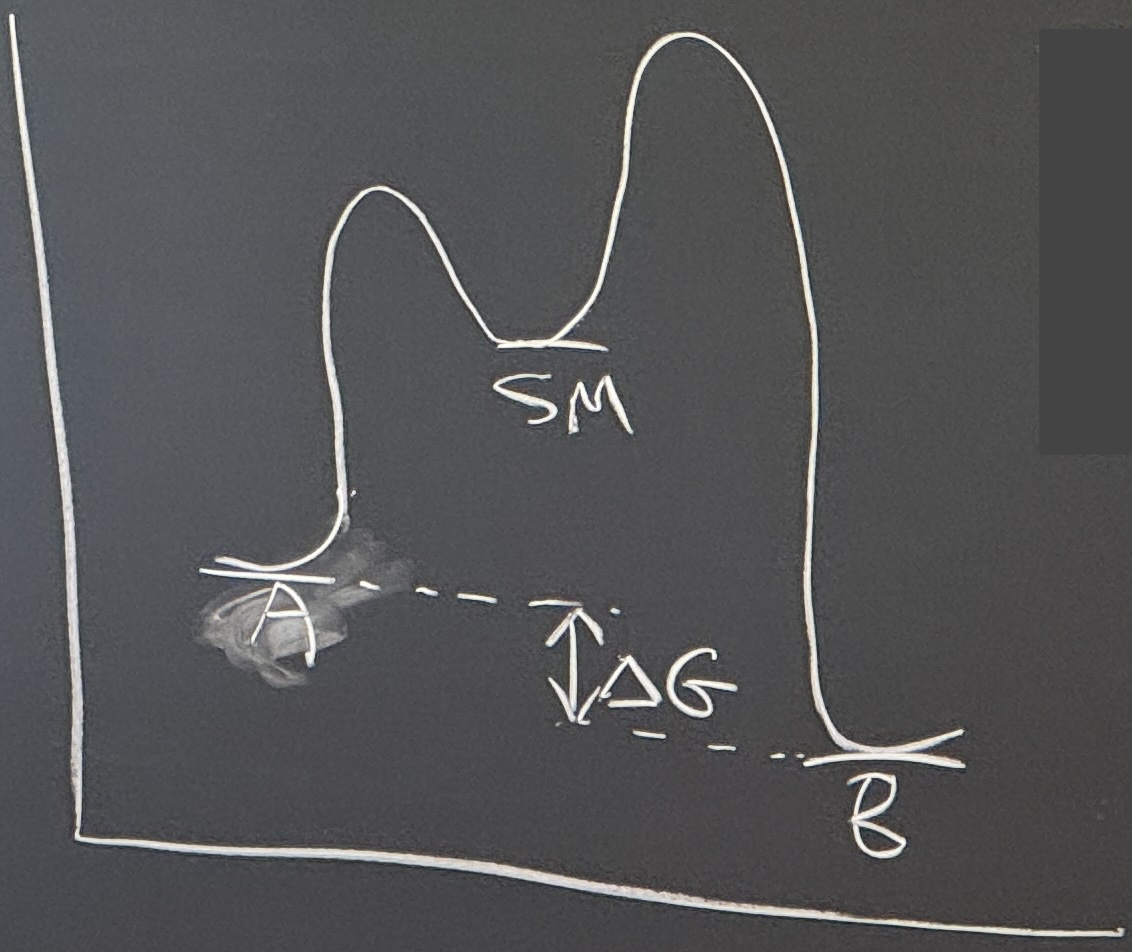
\includegraphics[width=0.2\linewidth]{EstabTherm.JPG}
        \caption{Energy variables relevant to thermodynamic selectivity.}
        \label{fig:EstabTherm}
    \end{figure}
    \begin{itemize}
        \item Key words: Thermodynamic = product = equilibrium.
        \item Relevant reaction coordinate.
        \begin{equation*}
            \ce{A <=>[$K_{\ce{A}}$] SM <=>[$K_{\ce{B}}$] B}
        \end{equation*}
        \begin{itemize}
            \item \ce{A} and \ce{B} form from a single common starting material (SM).
            \item The relevant equilibrium constants are $K_{\ce{A}}$ and $K_{\ce{B}}$.
        \end{itemize}
        \item $K_{\ce{A}}$ and $K_{\ce{B}}$ allow us to define the \textbf{selectivity} of this reaction as follows.
        \begin{equation*}
            \text{selectivity} = \frac{\cnc{A}}{\cnc{B}}
            = \frac{K_{\ce{A}}}{K_{\ce{B}}}
            =: \Keq
        \end{equation*}
        \item Energy diagram of a thermodynamically controlled reaction (Figure \ref{fig:EstabTherm}).
        \begin{itemize}
            \item In order for a reaction to be under thermodynamic control, all steps must be reversible, i.e., all intermediates must interconvert.
            \item $\Delta G$ is the difference in energy between the products.
            \item Recall from Gen Chem that $\Delta G=-RT\ln(\Keq)$ and hence $\Keq=\e[-\Delta G/RT]$.
        \end{itemize}
        \item Thermodynamic selectivity is very useful if all products are at very different energy levels.
        \item Example: Olefin isomerization can occur with great selectivity because one product can be much more stable than another.
    \end{itemize}
    \item \textbf{Selectivity} (of a reaction): The preference for one product (\ce{A}) over another (\ce{B}), where both \ce{A} and \ce{B} originate from a single common intermediate or starting material. \emph{Given by}
    \begin{equation*}
        \text{selectivity} := \frac{\cnc{A}}{\cnc{B}}
    \end{equation*}
    \item \textbf{Kinetic} (selectivity): Selecting for a certain product based on the differences in energies of competing transition states, i.e., by reaction rates.
    \begin{figure}[H]
        \centering
        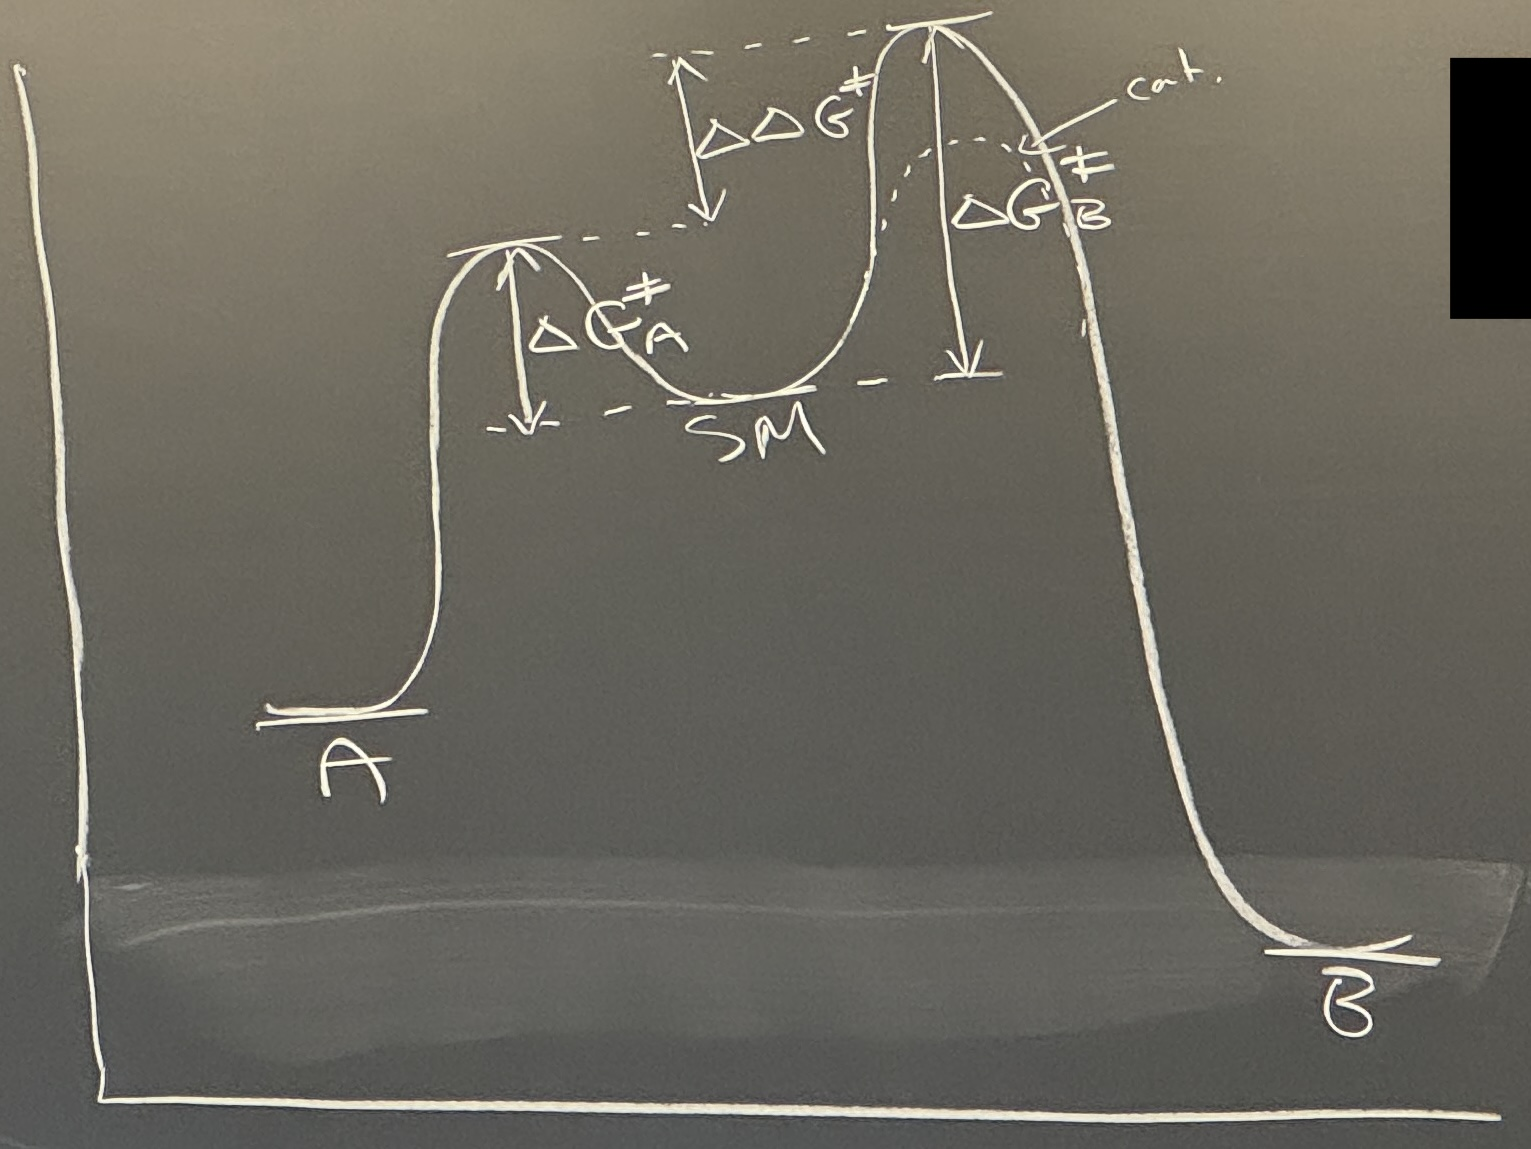
\includegraphics[width=0.35\linewidth]{EstabKin.JPG}
        \caption{Energy variables relevant to kinetic selectivity.}
        \label{fig:EstabKin}
    \end{figure}
    \begin{itemize}
        \item Key words: Kinetic = transition state = rate.
        \item Relevant reaction coordinate.
        \begin{equation*}
            \ce{A <-[$k_{\ce{A}}$] SM ->[$k_{\ce{B}}$] B}
        \end{equation*}
        \begin{itemize}
            \item As before, \ce{A} and \ce{B} form from a single common SM.
            \item The relevant rate constants are $k_{\ce{A}}$ and $k_{\ce{B}}$.
        \end{itemize}
        \item $k_{\ce{A}}$ and $k_{\ce{B}}$ allow us to define the selectivity of this reaction as follows.
        \begin{equation*}
            \text{selectivity} = \frac{\cnc{A}}{\cnc{B}}
            = \frac{k_{\ce{A}}}{k_{\ce{B}}}
        \end{equation*}
        \item Energy diagram of a kinetically controlled reaction (Figure \ref{fig:EstabKin}).
        \begin{itemize}
            \item $\Delta G_{\ce{A}}^\ddagger$ and $\Delta G_{\ce{B}}^\ddagger$ are the activation energies required to form the transition states from the SM to \ce{A} and \ce{B}, respectively.
            \item $\Delta\Delta G^\ddagger$ is then the difference between these transition states' activation energies.
            \item Recall from Gen Chem that $\Delta\Delta G^\ddagger=-RT\ln(k_{\ce{A}}/k_{\ce{B}})$.\footnote{This can be derived by dividing the Arrhenius equation for one reaction by the Arrhenius equation for the other reaction and rearranging.}
            \item Often, $k_{\ce{A}}/k_{\ce{B}}$ is equal to the relative rate $\krel$ of the two reactions (\ce{SM -> A} and \ce{SM -> B}).
            \begin{itemize}
                \item If \ce{A} and \ce{B} are enantiomers or diastereomers, $\krel$ often equals \textbf{er} or \textbf{dr}, respectively.
                \item Another consequence of the introduction of $\krel$ is that $\krel=\e[-\Delta\Delta G^\ddagger/RT]$.
            \end{itemize}
            \item Note that \emph{catalyzing} a pathway is a kinetic effect, corresponding to a lower activation barrier.
        \end{itemize}
        \item In contrast to thermodynamic equilibrium, the products formed here are formed irreversibly and do not interconvert.
        \item Kinetic control is more common than thermodynamic control.
        \begin{itemize}
            \item Reactions under thermodynamic control have largely been developed and optimized over the last 100 years, so kinetic control gives us a better handle in modern methods development.
            \item Everything about a catalytic cycle is based on kinetics! You're not changing the thermodynamics of \ce{CO2} upcycling; you're making it more energetically feasible.
        \end{itemize}
    \end{itemize}
    \item \textbf{Enantiomeric ratio}: The ratio of the (\emph{S})-enantiomer to the (\emph{R})-enantiomer. \emph{Denoted by} \textbf{er}.
    \begin{itemize}
        \item This is more mathematically useful than the enantiomeric excess (ee), so there's currently something of a push to phase out ee in favor of er.
        \item ee is still used primarily for historical reasons.
    \end{itemize}
    \item \textbf{Diasteriomeric ratio}: The ratio of one diastereomer to the other. \emph{Denoted by} \textbf{dr}.
    \item We now discuss a special type of kinetic control called \textbf{Curtin-Hammett kinetics}.
    \item \textbf{Curtin-Hammett} (kinetics): A kinetic regime characterized by two starting materials or intermediates that rapidly interconvert, causing the ratio of products (i.e., the selectivity) to depend only on the transition state energies. \emph{Also known as} \textbf{C/H}.
    \begin{figure}[H]
        \centering
        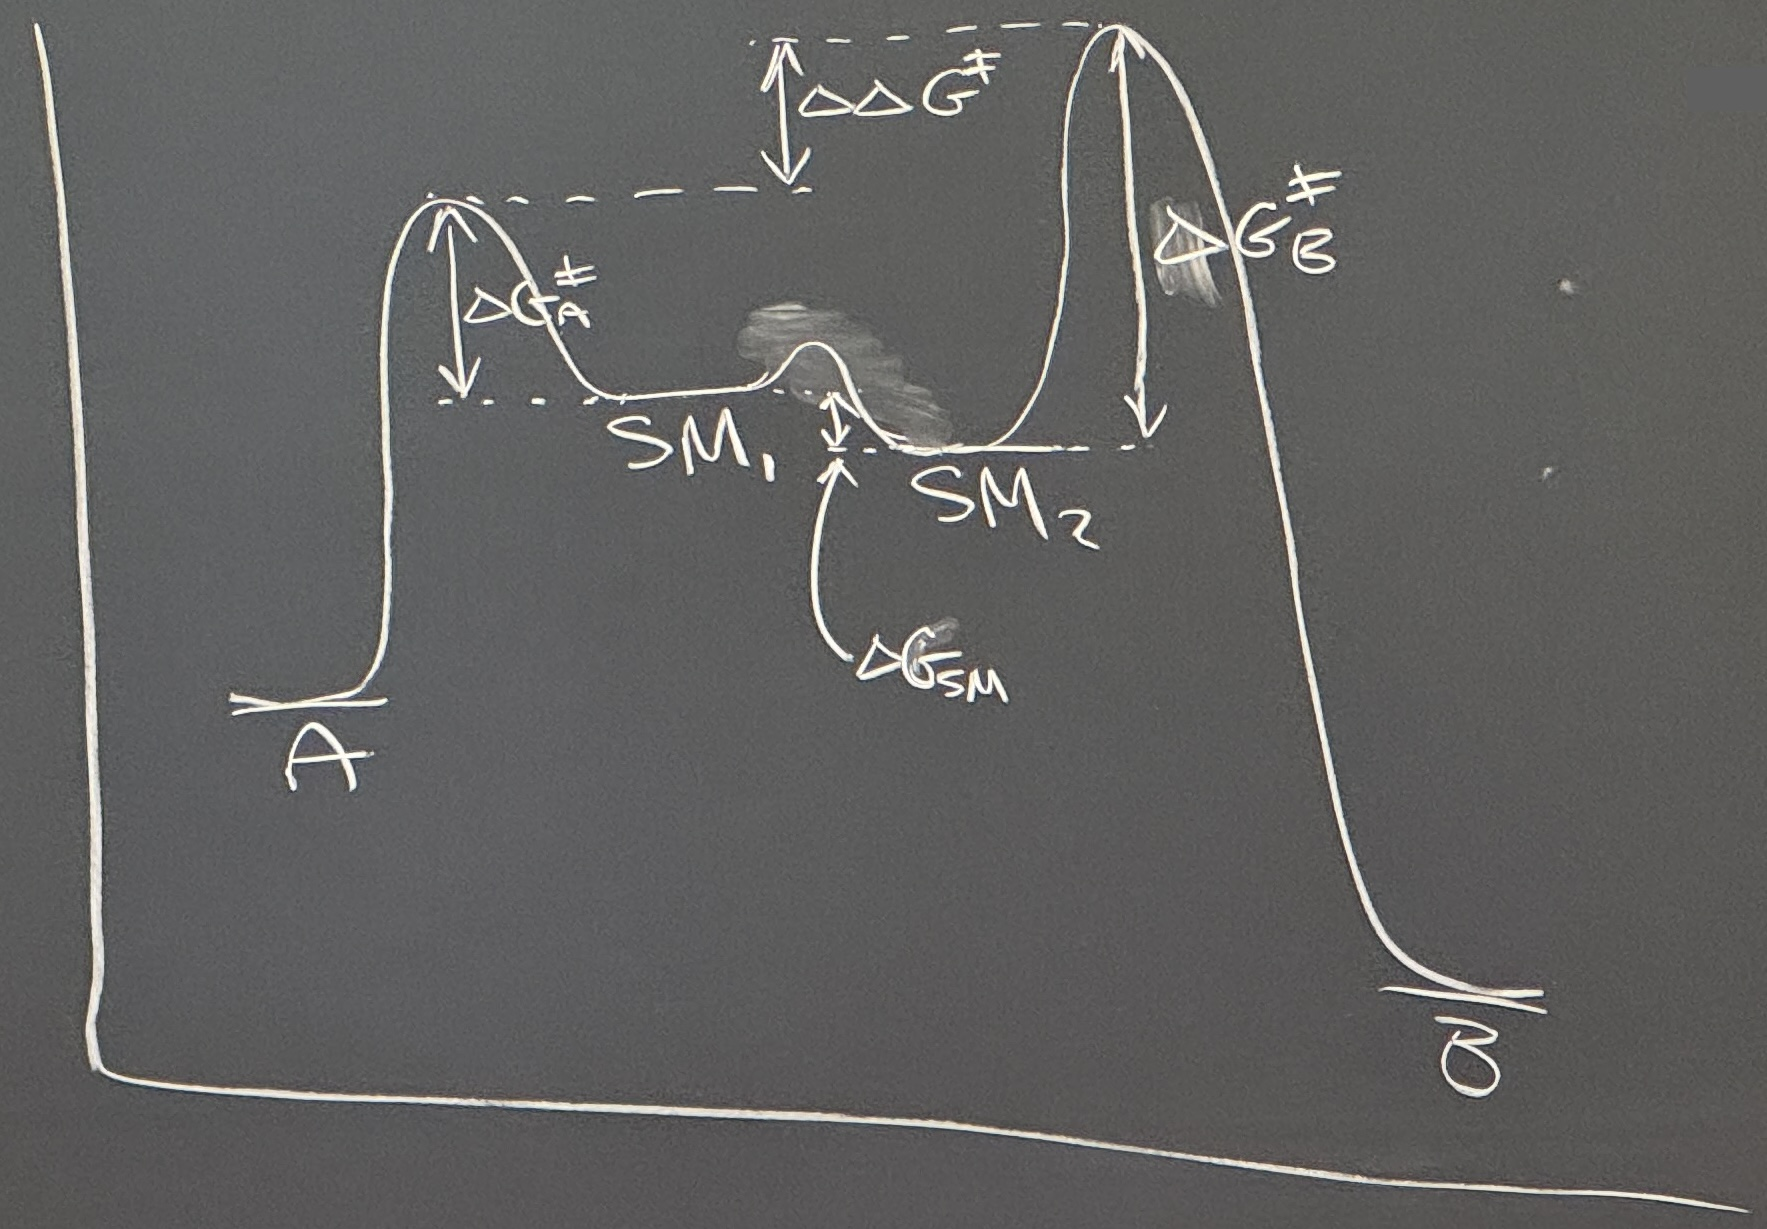
\includegraphics[width=0.35\linewidth]{EvarCH.JPG}
        \caption{Energy variables relevant to Curtin-Hammett kinetics.}
        \label{fig:EvarCH}
    \end{figure}
    \begin{itemize}
        \item In particular, the selectivity does \emph{not} depend on the energies of the starting materials.
        \item Relevant reaction coordinate.
        \begin{equation*}
            \ce{A <-[$k_{\ce{A}}$] SM1 <=>[$K_\text{SM}$][$k_\text{SM}$] SM2 ->[$k_{\ce{B}}$] B}
        \end{equation*}
        \begin{itemize}
            \item $k_\text{SM}$ must be big. Typically, it is approximately ten times faster than $k_{\ce{A}}$ or $k_{\ce{B}}$.
        \end{itemize}
        \item Working out the math, we get
        \begin{equation*}
            \text{selectivity} = \frac{\cnc{A}}{\cnc{B}}
            = \e[-\Delta\Delta G^\ddagger/RT]
        \end{equation*}
        \begin{itemize}
            \item Indeed, we see that in this regime, the selectivity \emph{mathematically} depends only on the relative energies of the transition states.
        \end{itemize}
        \item Energy diagram of a reaction under Curtin-Hammett kinetics (Figure \ref{fig:EvarCH}).
        \begin{itemize}
            \item Note that there is only a small energy barrier between \ce{SM1} and \ce{SM2} because we need fast interconversion.
        \end{itemize}
        \item Observe that the products are formed irreversibly and do not interconvert.
        \begin{itemize}
            \item Indeed, the SMs interconvert freely as long as they stay SMs, but once they go over their barrier to \ce{A} or \ce{B}, they do not continue to interconvert.
        \end{itemize}
    \end{itemize}
    \item Scenarios that manifest Curtin-Hammett kinetics.
    \begin{figure}[h!]
        \centering
        \begin{subfigure}[b]{0.33\linewidth}
            \centering
            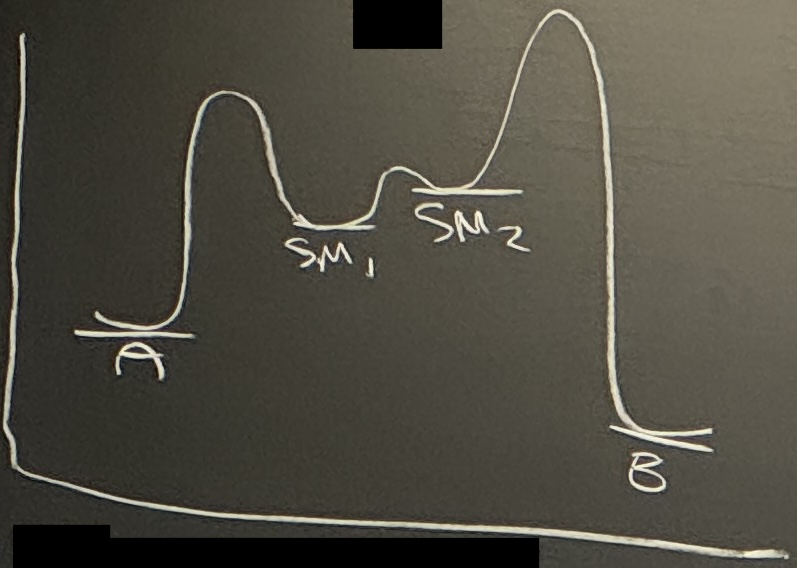
\includegraphics[width=0.79\linewidth]{CHscenarioa.JPG}
            \caption{More stable reacts more quickly.}
            \label{fig:CHscenarioa}
        \end{subfigure}
        \begin{subfigure}[b]{0.32\linewidth}
            \centering
            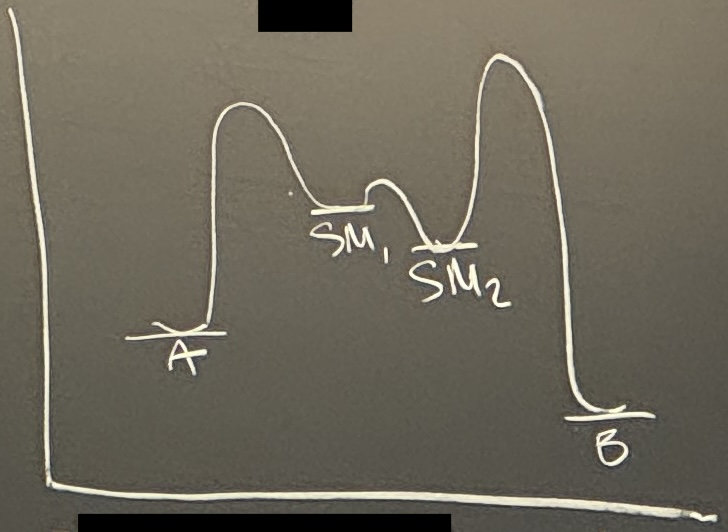
\includegraphics[width=0.8\linewidth]{CHscenariob.JPG}
            \caption{Less stable reacts more quickly.}
            \label{fig:CHscenariob}
        \end{subfigure}
        \begin{subfigure}[b]{0.33\linewidth}
            \centering
            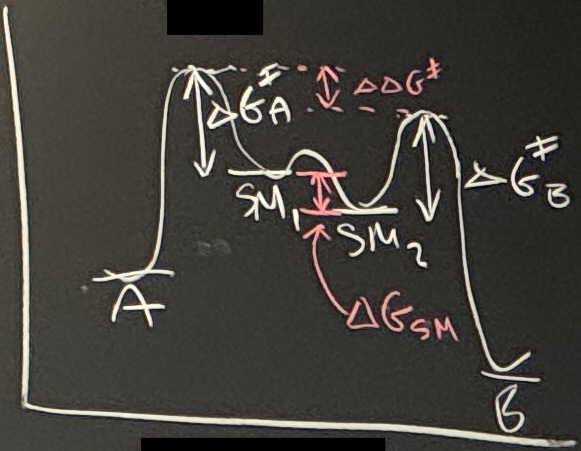
\includegraphics[width=0.74\linewidth]{CHscenarioc.JPG}
            \caption{Both react same.}
            \label{fig:CHscenarioc}
        \end{subfigure}
        \caption{Curtin-Hammett scenarios.}
        \label{fig:CHscenario}
    \end{figure}
    \begin{enumerate}
        \item The more stable starting material reacts more quickly (Figure \ref{fig:CHscenarioa}).
        \begin{itemize}
            \item Let \ce{SM1} be lower energy than \ce{SM2}, and let the \ce{SM1 -> A} transition state have a lower activation energy than the \ce{SM2 -> B} transition state.
            \item It follows that \ce{SM1} is thermodynamically favored. This means that we'll see more of it in solution: $\cnc{SM1}>\cnc{SM2}$.
            \item The lower activation energy to form \ce{A} (i.e., $\Delta G_{\ce{A}}^\ddagger<\Delta G_{\ce{B}}^\ddagger$) implies that \ce{A} is kinetically favored.
            \item The product ratio will not be equal to the starting material ratio.
            \begin{itemize}
                \item You might not even see \ce{SM2} among the starting materials; you might just think that \ce{SM1 -> A + B}.
            \end{itemize}
            \item Takeaway: It isn't always obvious when Curtin-Hammett kinetics are in effect.
        \end{itemize}
        \item The less stable starting material reacts more quickly (Figure \ref{fig:CHscenariob}).
        \begin{itemize}
            \item Let \ce{SM1} be higher energy than \ce{SM2}, and let the \ce{SM1 -> A} transition state have a lower activation energy than the \ce{SM2 -> B} transition state.
            \item It follows that \ce{SM2} is thermodynamically favored. This means that we'll see more of it in solution: $\cnc{SM2}>\cnc{SM1}$.
            \item The lower activation energy to form \ce{A} (i.e., $\Delta G_{\ce{A}}^\ddagger<\Delta G_{\ce{B}}^\ddagger$) implies that \ce{A} is kinetically favored.
            \item The less stable starting material is kinetically favored to react.
            \item Takeaway: All the reactivity goes through \ce{SM1}, even though we might not even see \ce{SM1}; you might just think that \ce{SM2 -> A + B}.
            \item This is classic Curtin-Hammett kinetics, wherein the product we observe is from the starting material we don't observe.
            \begin{itemize}
                \item Results like this can be confusing because the SM we put in the flask doesn't look like it'd give the product we see.
                \item This contrasts with Scenario 1, wherein the SM we see logically leads to our product \ce{A}, and all we miss is that there's a secret equilibrium that helps us get to \ce{B}.
            \end{itemize}
        \end{itemize}
        \item Both starting materials react equally quickly (Figure \ref{fig:CHscenarioc}).
        \begin{itemize}
            \item Let \ce{SM1} be higher energy than \ce{SM2}, and let the \ce{SM1 -> A} and \ce{SM2 -> B} transition states have identical activation energies (i.e., $\Delta G_{\ce{A}}^\ddagger=\Delta G_{\ce{B}}^\ddagger$).
            \item We call this \textbf{ground state control}.
            \begin{itemize}
                \item Thus, $\Delta G_{\ce{SM}}$ suddenly predicts our products; not because it actually does but because $\Delta\Delta G^\ddagger=\Delta G_{\ce{SM}}$.
                \item To reiterate: $\Delta\Delta G^\ddagger$ still controls selectivity; it just happens that it equals $\Delta G_{\ce{SM}}$.
            \end{itemize}
            \item Because $\Delta\Delta G^\ddagger=\Delta G_{\ce{SM}}$, we can work out mathematically that the selectivity happens to be the following (even though we still have C/H kinetics).
            \begin{equation*}
                \text{selectivity} = \frac{\cnc{A}}{\cnc{B}}
                = \frac{\cnc{SM1}}{\cnc{SM2}}
            \end{equation*}
            \item This regime often arises when \ce{A} and \ce{B} are really similar and hence have similar transition states (e.g., if \ce{A} and \ce{B} are enantiomers or diastereomers with far apart stereogenic centers).
        \end{itemize}
    \end{enumerate}
    \item It's our job as the responsible scientist to account for the full kinetic picture, even when it may not provide us much additional information!
    \begin{itemize}
        \item Indeed, the reactions that are the most interesting to develop are the ones that fall in this C/H regime because they have the most subtle reactivity.
    \end{itemize}
    \item Let's now look at some examples.
    \begin{itemize}
        \item Pay attention, because this is going to be a super useful skill for grad school and beyond!!
    \end{itemize}
    \item Example: Nitrogen rapidly epimerizes while a \emph{tert}-butyl group locks the chair in place.
    \begin{figure}[h!]
        \centering
        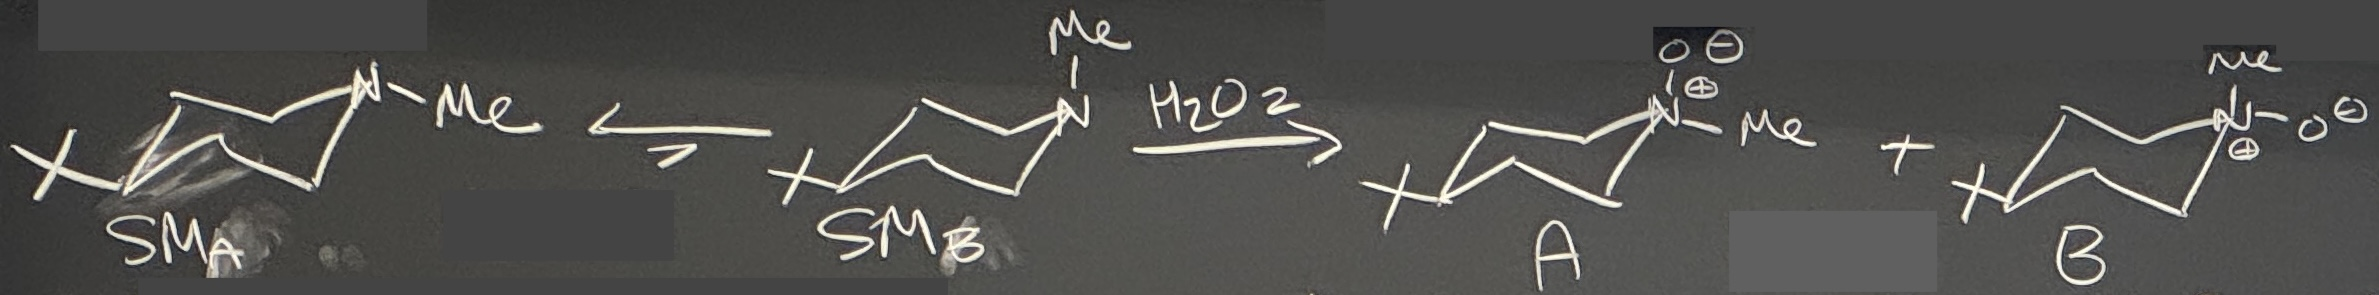
\includegraphics[width=0.6\linewidth]{CHepimers.JPG}
        \caption{Curtin-Hammett kinetics: Kinetically trapping epimers.}
        \label{fig:CHepimers}
    \end{figure}
    \begin{itemize}
        \item This epimerization (a \textbf{nitrogen inversion}) occurs fast relative to product formation.
        \item It puts \ce{SM_A} and \ce{SM_B} in a $98:2$ ratio.
        \item Either epimer can react with \ce{H2O2} to form the \emph{N}-oxo products in a $5:95$ ($\ce{A}:\ce{B}$) ratio.
        \item This is an example of Scenario 2 (Figure \ref{fig:CHscenariob}).
        \begin{itemize}
            \item Your first thought might be that the oxidation occurs with inversion of stereochemistry. This is a great first thought.
            \item But then you have to ask about alternate scenarios, and you should think about decoupled Curtin-Hammett steps wherein you're just kinetically trapping the epimers.
        \end{itemize}
    \end{itemize}
    \item Example: Axial and equatorial tosylates equilbriate before E\textsubscript{2} elimination to form a double bond.
    \begin{figure}[H]
        \centering
        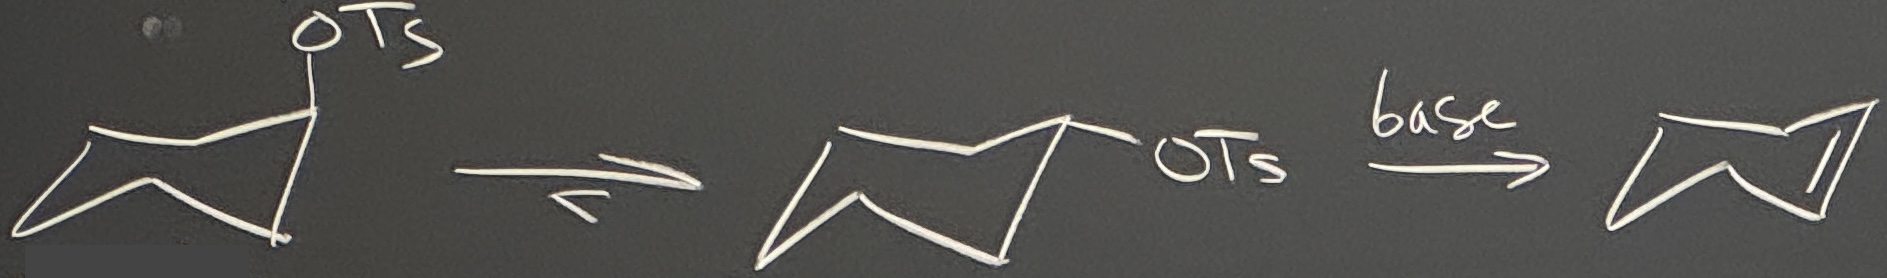
\includegraphics[width=0.4\linewidth]{CHelim.JPG}
        \caption{Curtin-Hammett kinetics: Elimination.}
        \label{fig:CHelim}
    \end{figure}
    \begin{itemize}
        \item Let \ce{SM_A} be the axial tosylate (on the left), and let \ce{SM_B} be the equatorial tosylate (on the right).
        \item Because of the large steric bulk of the tosylate group and hence its disfavored 1,3-diaxial interactions, \ce{SM_A} and \ce{SM_B} occur in a $1:14$ ratio.
        \item However, \ce{SM_A} has hydrogens antiperiplanar to it, so it reacts faster ($\krel=70$).
        \item So to recap: \ce{SM_B} is preferred, but the product comes from \ce{SM_A}. Therefore, this must be another example of Scenario 2 (Figure \ref{fig:CHscenariob}).
    \end{itemize}
    \item Example: \emph{trans} and \emph{cis} alkenes react via bromination to form a \emph{trans}- and \emph{cis}-dibromide.
    \begin{figure}[h!]
        \centering
        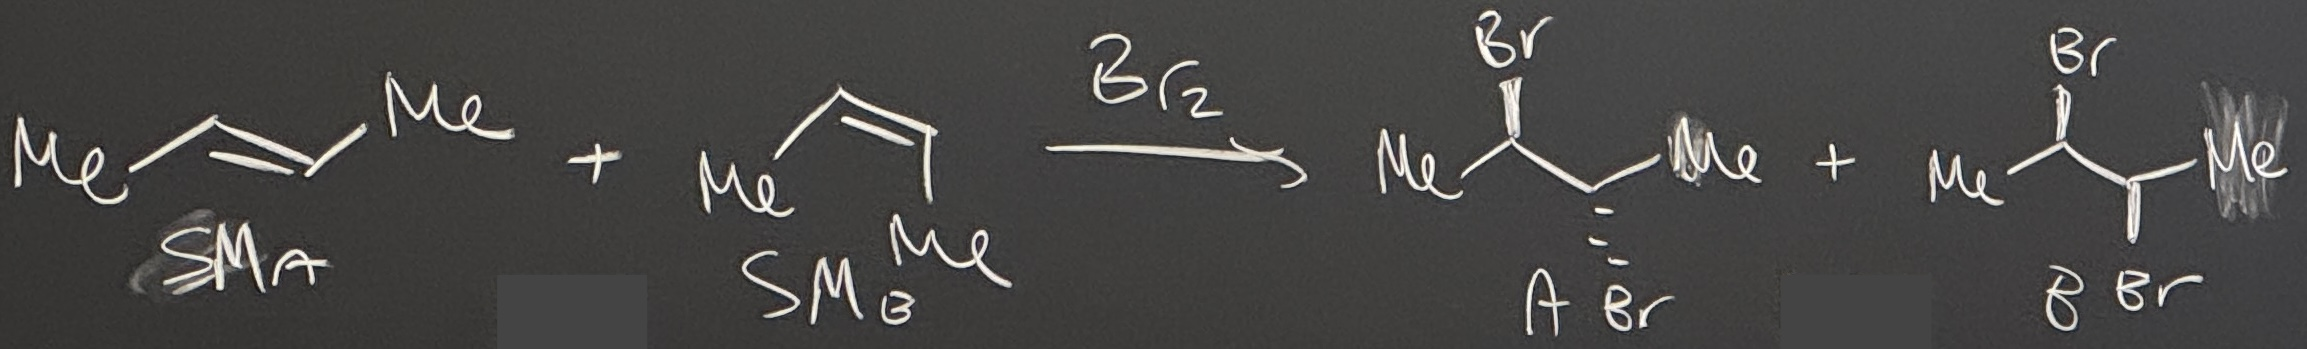
\includegraphics[width=0.5\linewidth]{CHgeometric.JPG}
        \caption{Curtin-Hammett kinetics: Bromination of geometric isomers.}
        \label{fig:CHgeometric}
    \end{figure}
    \begin{itemize}
        \item We have a $1:1$ mixture of SMs, and we form a $1:1$ mixture of products.
        \item Thus, based on the selectivity equation, it looks like this could be a candidate for Scenario 3. However, this is not C/H because the SMs do not interconvert! Rather, this is a case of a kinetic quench, which we'll cover next.
    \end{itemize}
    \item Learn C/H because we will see a lot of it on PSet 2.
    \item Kinetic quench (not C/H).
    \begin{figure}[h!]
        \centering
        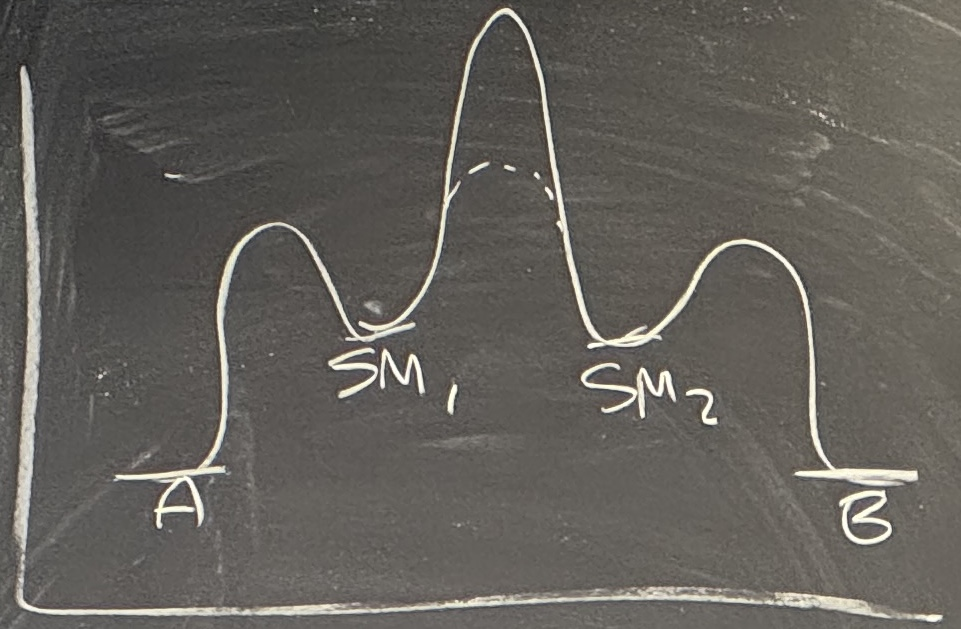
\includegraphics[width=0.25\linewidth]{EvarKQ.JPG}
        \caption{Energy variables relevant to a kinetic quench.}
        \label{fig:EvarKQ}
    \end{figure}
    \begin{itemize}
        \item Here, the \ce{SM1 <=> SM2} interconversion is slower than product formation.
        \item Thus, the ratio of starting materials equals the ratio of products, as follows.
        \begin{equation*}
            \text{product ratio} = \frac{\cnc{A}}{\cnc{B}}
            = \frac{\cnc{SM1}}{\cnc{SM2}}
        \end{equation*}
        \item This is basically a case of two isolated systems (\ce{SM1 -> A} and \ce{SM2 -> B}).\footnote{Could I come up with one-pot reactions where you have two different starting materials under kinetic quench form two different products and then those products react??}
        \pagebreak
        \item One tricky thing: When the rate of interconversion approximately equals the rate of product formation (Masha shows this regime with the dotted line in Figure \ref{fig:EvarKQ}).
        \begin{itemize}
            \item In this case, the product ratio is difficult to predict!
            \item That's real, messy science.
            \item When you encounter such a regime, either you change something to make it simpler, or you do a Wendlandt-style deep dive on the full mechanism where you uncover the secrets of the universe and then publish a bunch of \emph{Science} papers.
            \item "Alison's the master of these really hairy and difficult kinetic pictures and disentangling them and adding to our understanding of chemistry overall."
        \end{itemize}
    \end{itemize}
    \item Example of kinetic quench: Protonating two different epimers of an amine.
    \begin{figure}[h!]
        \centering
        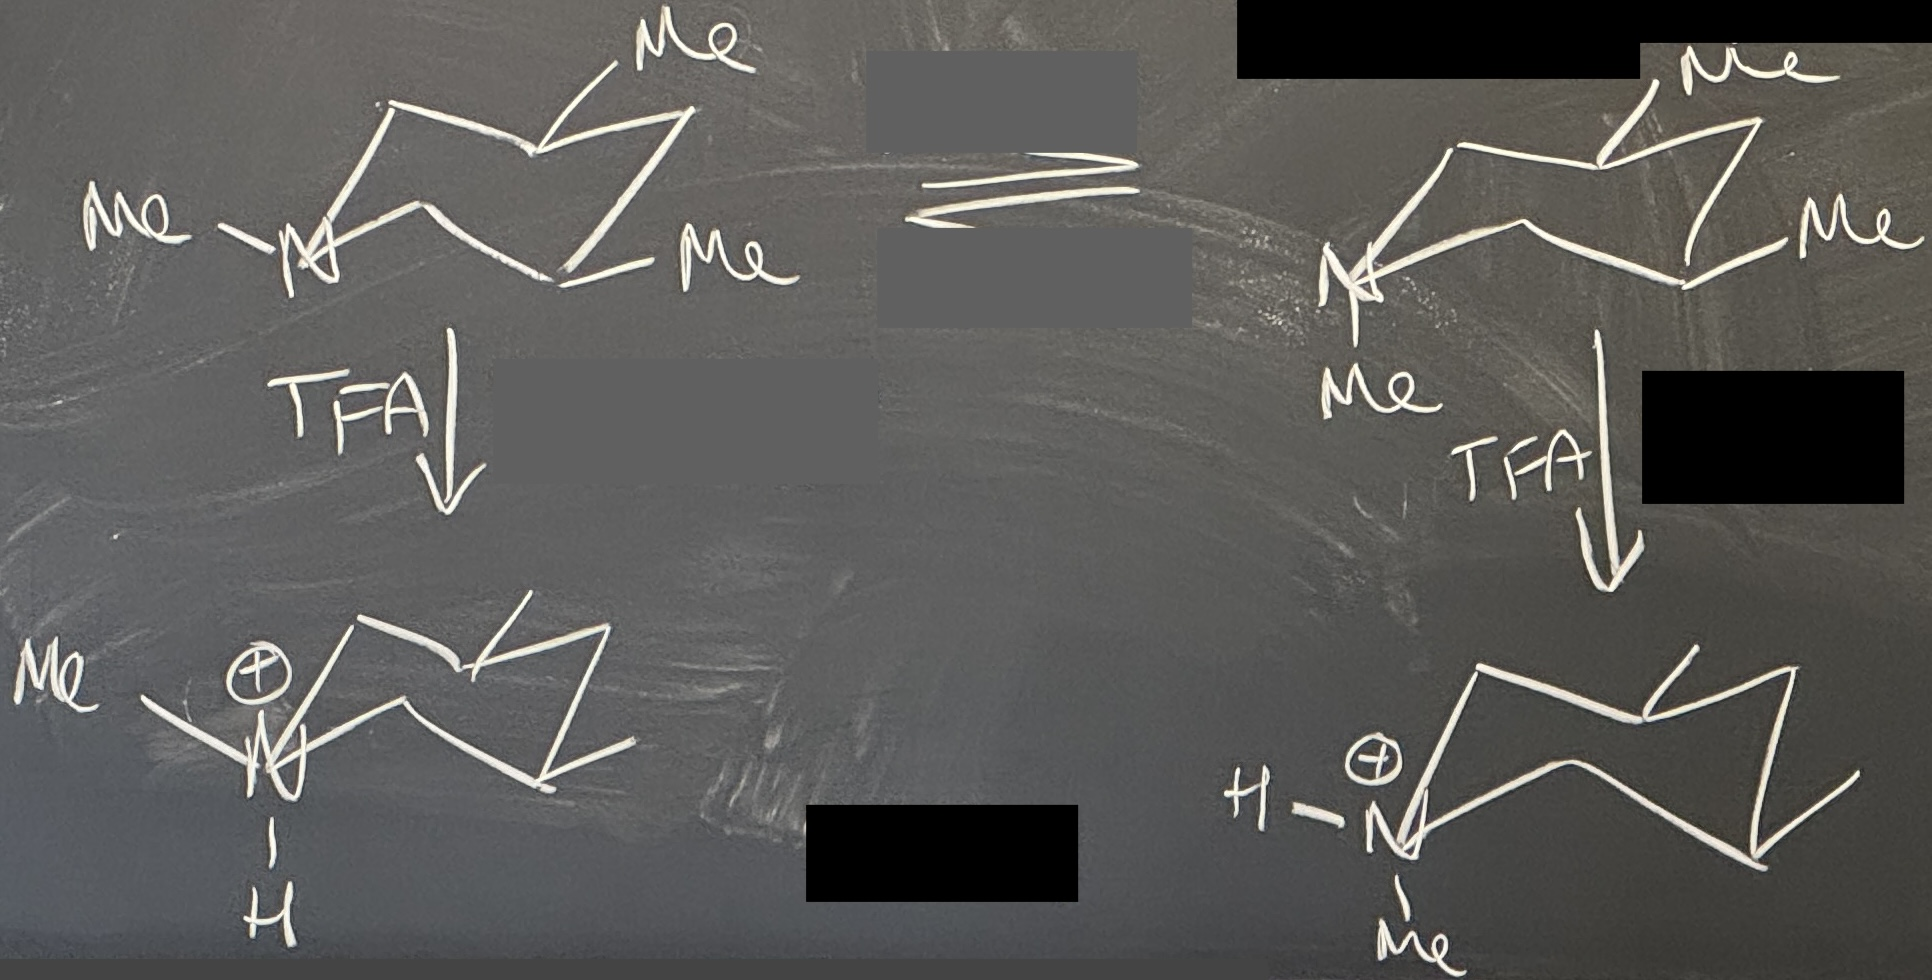
\includegraphics[width=0.45\linewidth]{KQprotonation.JPG}
        \caption{Kinetic quench: Protonation.}
        \label{fig:KQprotonation}
    \end{figure}
    \begin{itemize}
        \item The epimer with the equatorial methyl occurs in a $>15:1$ ratio.
        \item Epimerization occurs relatively slowly, protonation of the equatorial lone pair occurs fast, and protonation of the axial lone pair is even \emph{faster} than protonation of the equatorial one.
        \begin{itemize}
            \item What is "fast" and "slow" is all relative! Usually, nitrogen inversion is fast, but proton transfer (PT) to nitrogen is even faster.
        \end{itemize}
        \item However, the product ratio is also $>15:1$, just like the SM ratio. To reiterate, this is because we're not interconverting between our starting materials.
    \end{itemize}
    \item Moving on, let's discuss the \textbf{principle of microscopic reversibility}.
    \item \textbf{Principle of microscopic reversibility}: The lowest energy path connecting two intermediates is the same, regardless of the direction in which the reaction proceeds.
    \begin{itemize}
        \item Basically, if you propose a mechanism from \ce{A -> B}, the same mechanism (in reverse) has to be true for \ce{B -> A}.
        \item If we proceed through a certain transition state in one direction, we cannot proceed through a different transition state on the way back.
        \item Really useful to probe kinetically silent steps.
    \end{itemize}
    \item A cool example of using the principle of microscopic reversibility to see which mechanism is operative (Figure \ref{fig:MicroReverMech}).
    \begin{figure}[h!]
        \centering
        \begin{subfigure}[b]{\linewidth}
            \centering
            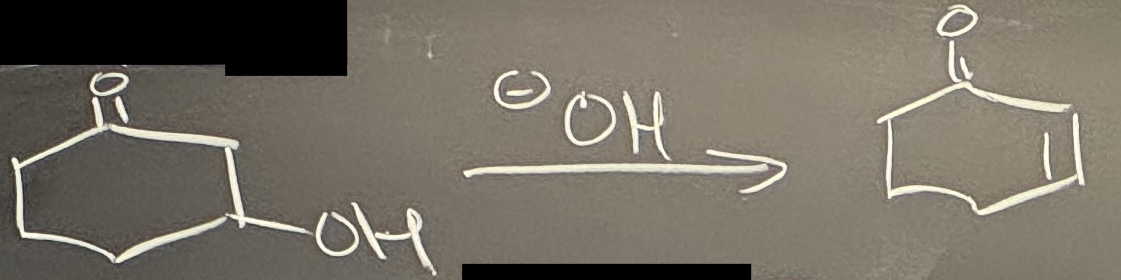
\includegraphics[width=0.25\linewidth]{MicroReverMecha.JPG}
            \caption{An elimination reaction.}
            \label{fig:MicroReverMecha}
        \end{subfigure}\\[2em]
        \begin{subfigure}[b]{0.49\linewidth}
            \centering
            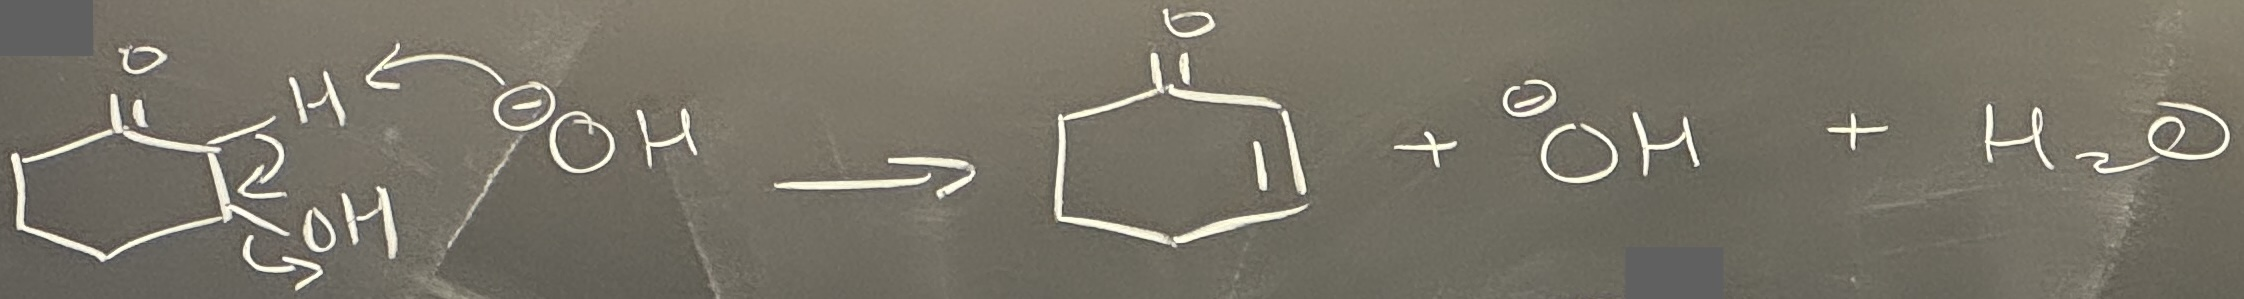
\includegraphics[width=0.95\linewidth]{MicroReverMechb.JPG}
            \caption{E\textsubscript{2} mechanism.}
            \label{fig:MicroReverMechb}
        \end{subfigure}
        \begin{subfigure}[b]{0.49\linewidth}
            \centering
            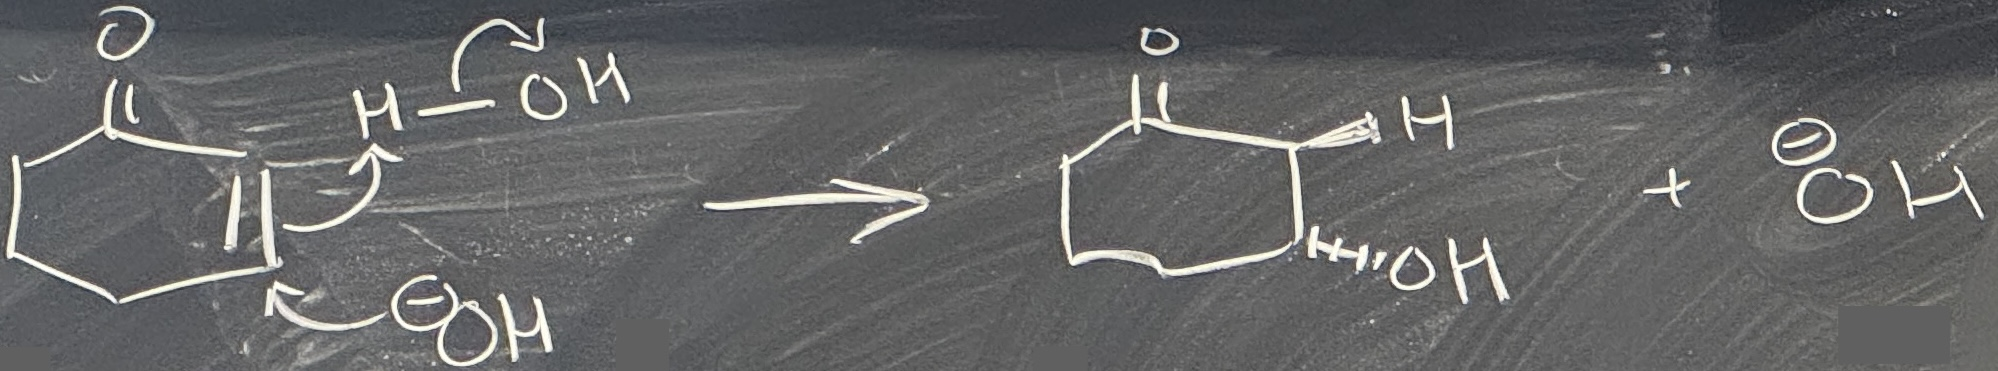
\includegraphics[width=0.82\linewidth]{MicroReverMechc.JPG}
            \caption{Retro-E\textsubscript{2} mechanism.}
            \label{fig:MicroReverMechc}
        \end{subfigure}\\[2em]
        \begin{subfigure}[b]{0.49\linewidth}
            \centering
            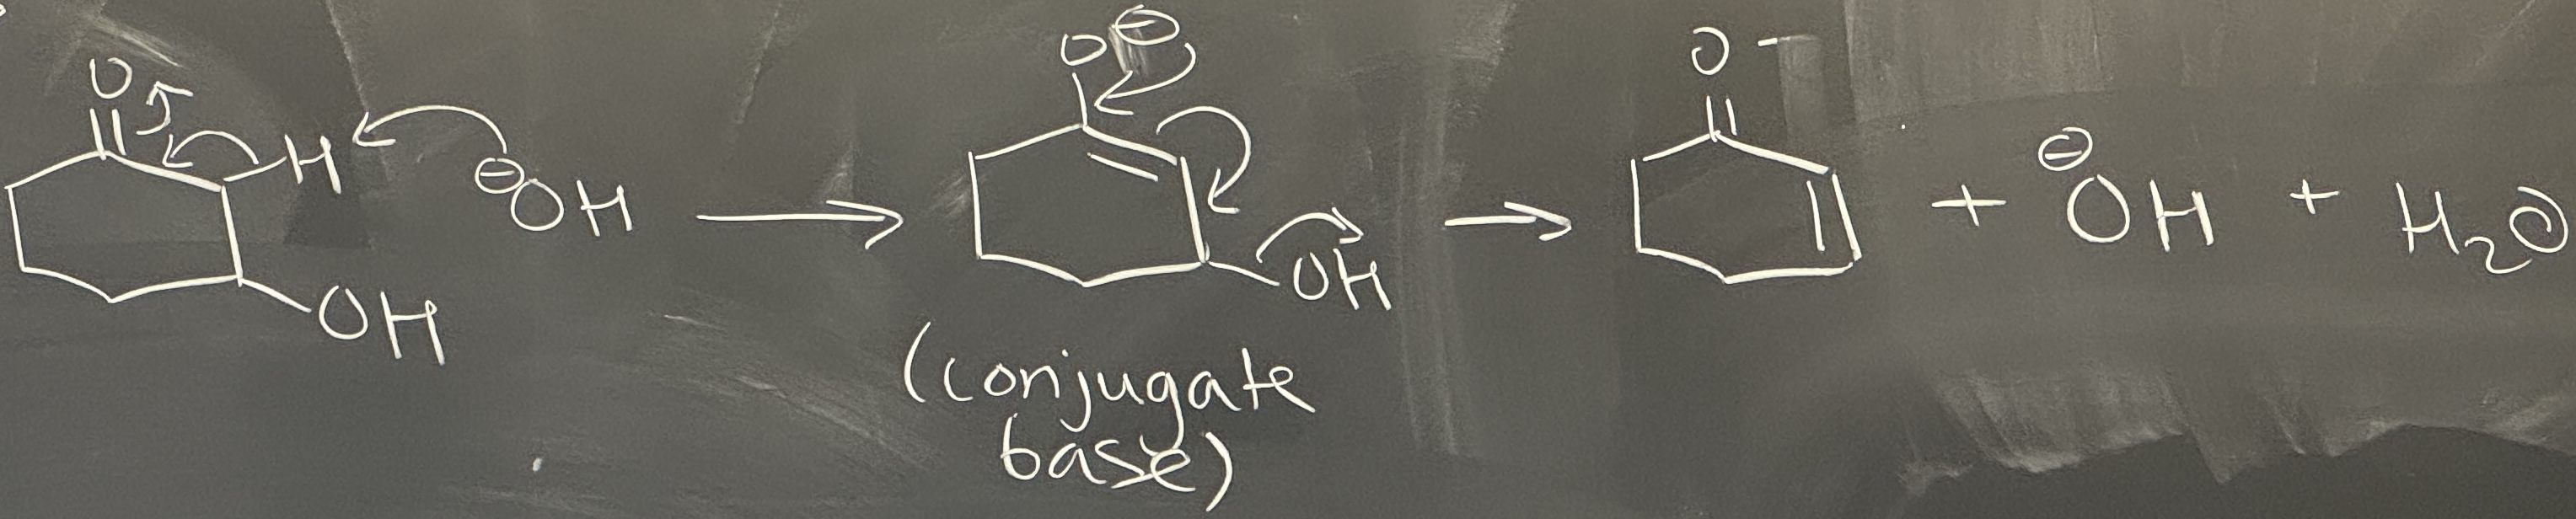
\includegraphics[width=\linewidth]{MicroReverMechd.JPG}
            \caption{E\textsubscript{1}CB mechanism.}
            \label{fig:MicroReverMechd}
        \end{subfigure}
        \begin{subfigure}[b]{0.49\linewidth}
            \centering
            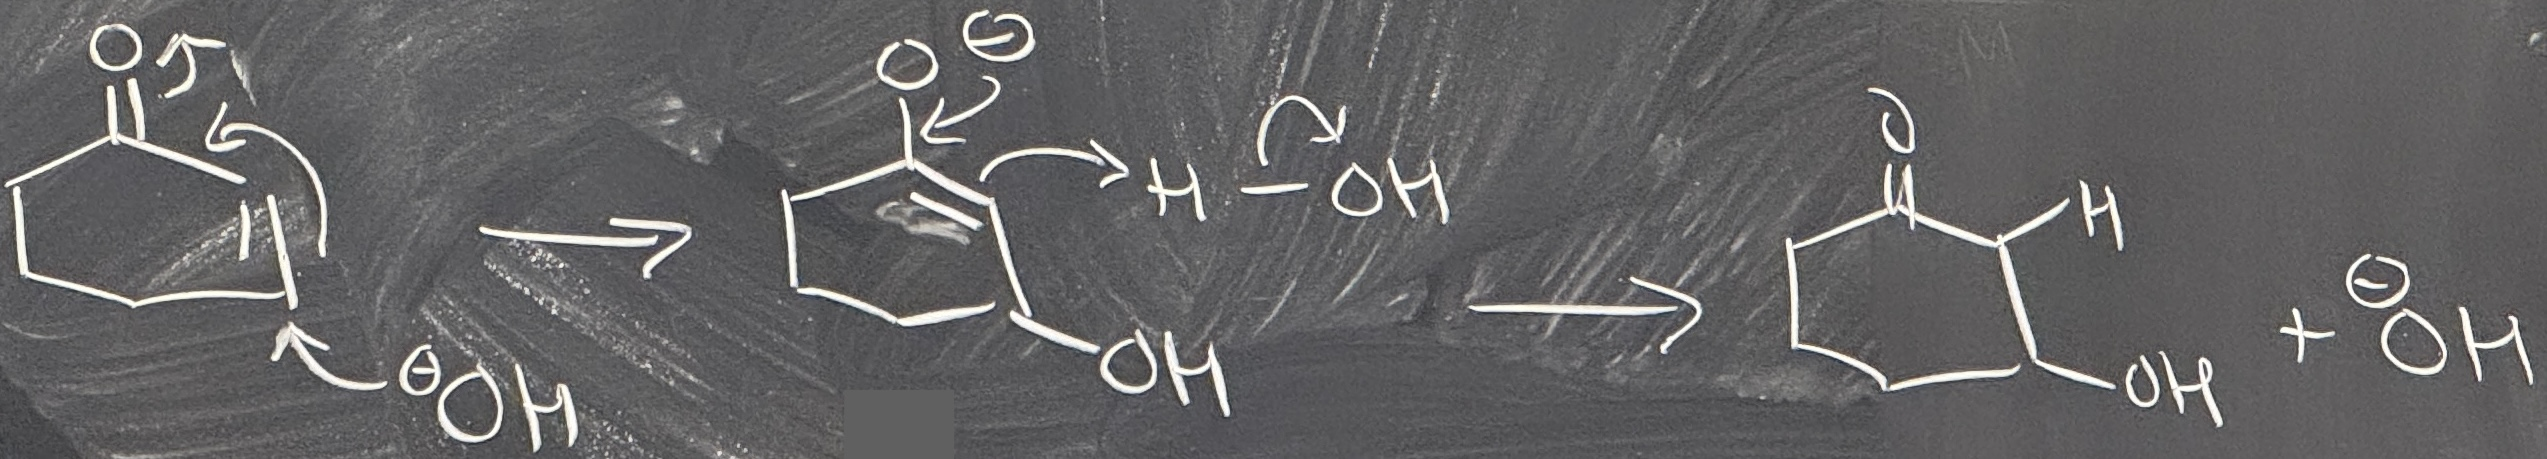
\includegraphics[width=0.95\linewidth]{MicroReverMeche.JPG}
            \caption{Retro-E\textsubscript{1}CB mechanism.}
            \label{fig:MicroReverMeche}
        \end{subfigure}
        \caption{Microscopic reversibility to differentiate plausible mechanisms.}
        \label{fig:MicroReverMech}
    \end{figure}
    \begin{itemize}
        \item Consider the elimination of a $\beta$-hydroxyketone to form an enone (Figure \ref{fig:MicroReverMecha}).
        \item Is the mechanism E\textsubscript{2} (Figure \ref{fig:MicroReverMechb}) or \textbf{E\textsubscript{1}CB} (Figure \ref{fig:MicroReverMechd})?
        \item How can we determine the better mechanism? Consider the reverse reactions!
        \begin{itemize}
            \item Retro-E\textsubscript{2} (Figure \ref{fig:MicroReverMechc}): A one-step forward reaction for E\textsubscript{2} means a one-step reverse reaction, wherein \ce{HO-} adds in, the olefin grabs a proton from water, and \ce{HO-} leaves.
            \item Retro-E\textsubscript{1}CB (Figure \ref{fig:MicroReverMeche}): This time, a two-step reverse reaction is implied. First, we kick electron density all the way up to oxygen, and second, we kick arrows back down to grab a proton.
        \end{itemize}
        \item Which reverse mechanism is more plausible?
        \begin{itemize}
            \item In Figure \ref{fig:MicroReverMechc}, we need a termolecular transition state (which is possible, but rare). However, we'd also form only the anti product, and this is flatly inconsistent with experiment.
            \item In Figure \ref{fig:MicroReverMeche}, we have a conjugate addition step followed by an enolate protonation step, both of which are very typical reactions.
            \begin{itemize}
                \item Molecular orbital theory also implies that the electrons push all the way up through the conjugated system to the oxygen in a concerted step upon nucleophilic addition at the B\"{u}rgi-Dunitz angle, like in 5.13!
            \end{itemize}
        \end{itemize}
        \item Now remember that the more reasonable mechanism must follow the same steps in the forward and reverse direction.
        \begin{itemize}
            \item Thus, more reasonable in reverse implies more reasonable in forward!
        \end{itemize}
        \item Conclusion: E\textsubscript{1}CB wins!
    \end{itemize}
    \item \textbf{Elimination unimolecular conjugate base}: Just a type of E1 that happens with an acidic proton. \emph{Also known as} \textbf{E\textsubscript{1}CB}.
    \begin{itemize}
        \item You draw the formation of a conjugate base (i.e., the conjugate base of the SM "acid") followed by the elimination of something.
    \end{itemize}
    \item That wraps it up for microscopic reversibility; let's now move onto another principle.
    \item \textbf{Reactivity-selectivity principle}: It is often observed that a more reactive reactant, intermediate, or reagent corresponds to a less selective reaction.
    \begin{itemize}
        \item When we say "more reactive," we typically mean higher energy, more exothermic, etc.
        \item This happens because the transition states to different products tend to resemble this higher energy intermediate per the \textbf{Hammond postulate}.
        \item It follows since the transition state does not resemble the products that it is less sensitive to differences in product energy, so it is harder for the transition state to differentiate between products, so the reaction is less selective.
    \end{itemize}
    \item \textbf{Hammond postulate}: The transition state is most similar in structure to the higher energy intermediate.
    \item Example of the reactivity-selectivity principle: Radical halogenation.
    \begin{figure}[h!]
        \centering
        \footnotesize
        \schemestart
            \chemfig{-[:30](-[2])-[:-30]-[:30]}
            \arrow(.-10--){->[\ce{X2}][$h\nu$]}
            \chemfig{-[:30](-[:110])(-[:70]X)-[:-30]-[:30]}
            \+{,,0.7em}
            \chemfig{-[:30](-[2])-[:-30](-[6]X)-[:30]}
            \+
            \chemfig{-[:30](-[2]-[:30]X)-[:-30]-[:30]}
            \+
            \chemfig{-[:30](-[2])-[:-30]-[:30]-[:-30]X}
        \schemestop
        \caption{Reactivity-selectivity principle in radical halogenation.}
        \label{fig:reactSelect}
    \end{figure}
    \begin{itemize}
        \item This reaction yields 1 tertiary product, 2 different secondary products, and 1 primary product.
    \end{itemize}
    \item The reaction in Figure \ref{fig:reactSelect} forms diffferent product distributions with different halogens.
    \begin{table}[h!]
        \centering
        \small
        \renewcommand{\arraystretch}{1.2}
        \setchemfig{atom sep=1em,bond offset=1pt,fixed length=false,atom style={font=\tiny},bond style=thick}
        \begin{tabular}{c|cccc}
             & \chemfig{-[:30](-[:110])(-[:70]\textbf{X})-[:-30]-[:30]}
                & \chemfig{-[:30](-[2])-[:-30](-[6]\textbf{X}-[6,0.5,,,opacity=0])-[:30]}
                & \chemfig{-[:30](-[2]-[:30]\textbf{X})-[:-30]-[:30]}
                & \chemfig{-[:30](-[2])-[:-30]-[:30]-[:-30]\textbf{X}}\\
            \hline
            $\bm{\textbf{X}=\textbf{Cl}}$ \textbf{(\%)} & 28 & 35 & 24 & 12\\
            $\bm{\textbf{X}=\textbf{Br}}$ \textbf{(\%)} & 90 & 9 & $<1$ & $<1$\\
        \end{tabular}
        \caption{Product distribution in radical bromination vs. chlorination.}
        \label{tab:reactSelect}
    \end{table}
    \begin{itemize}
        \item Evidently, \ce{Br*} is more selective than \ce{Cl*}.
    \end{itemize}
    \item Why? Consider BDEs in the selectivity-determining propagation step wherein a halide radical creates an alkyl radical and \ce{HCl}.
    \begin{figure}[h!]
        \centering
        \begin{subfigure}[b]{0.35\linewidth}
            \centering
            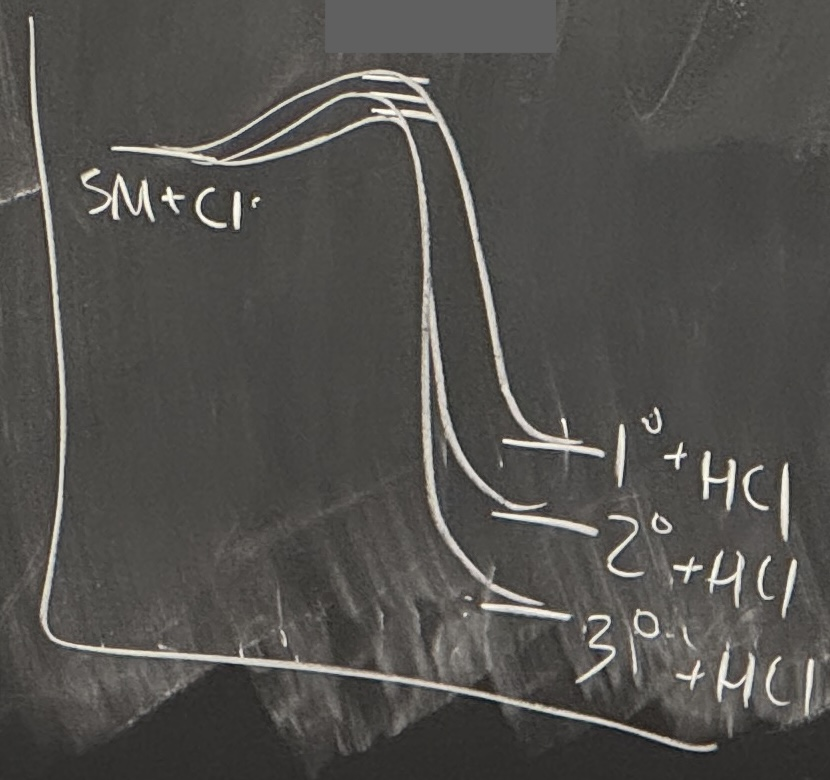
\includegraphics[width=0.7\linewidth]{Hammonda.JPG}
            \caption{Chlorination energy diagram.}
            \label{fig:Hammonda}
        \end{subfigure}
        \begin{subfigure}[b]{0.35\linewidth}
            \centering
            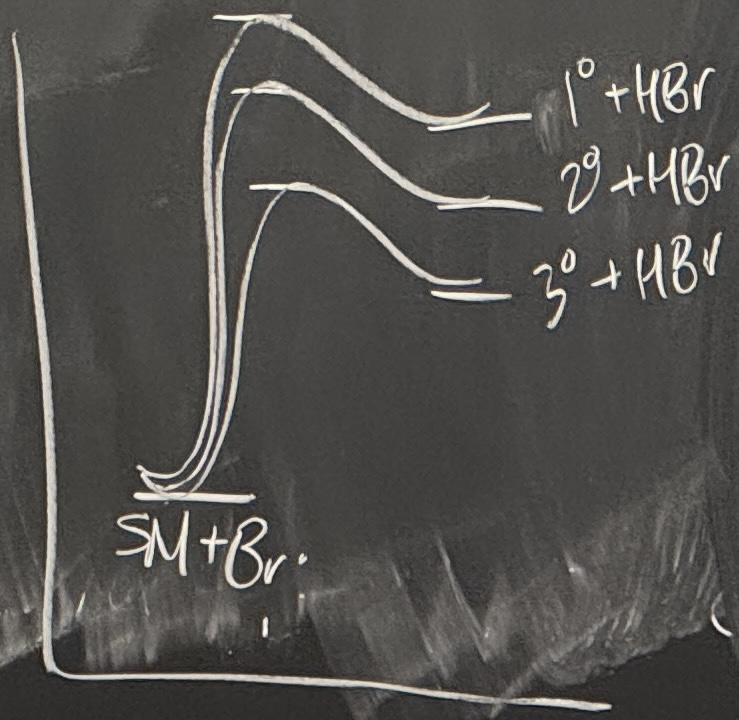
\includegraphics[width=0.68\linewidth]{Hammondb.JPG}
            \caption{Bromination energy diagram.}
            \label{fig:Hammondb}
        \end{subfigure}
        \caption{The Hammond postulate explains the reactivity-selectivity principle.}
        \label{fig:Hammond}
    \end{figure}
    \begin{itemize}
        \item In radical chlorination: \ce{C-H} has a BDE of \kcal{98} and \ce{H-Cl} has a BDE of \kcal{103}.
        \begin{itemize}
            \item Thus, the reaction is exothermic with $\Delta H=-\kcal{5}$.
            \item Then per the reactivity-selectivity principle, we have a high-energy intermediate. This will lead to three energetically close transition states that unselectively determine the product (Figure \ref{fig:Hammonda}).
        \end{itemize}
        \item In radical bromination: \ce{C-H} has a BDE of \kcal{98} and \ce{H-Br} has a BDE of \kcal{87}.
        \begin{itemize}
            \item Thus, the reaction is endothermic with $\Delta H=\kcal{11}$.
            \item Then per the reactivity-selectivity principle, we have a low-energy intermediate. This will lead to three energetically distinct transition states that resemble the product more and hence selectively determine it (Figure \ref{fig:Hammondb}).
        \end{itemize}
        \item The reactivity-selectivity principle is useful to understand and many-times true, but there are also many exceptions.
        \begin{itemize}
            \item Example exception: If there are more complicated mechanistic relationships between the SMs and transition states.
        \end{itemize}
        \item See Figure 3.4 of \textcite{bib:CHEM22100Notes}!
    \end{itemize}
    \item Practical aspects of selectivity (will come up on our quals).
    \begin{itemize}
        \item Numbers worth knowing.
        \item We'll go over this in the Lecture 10 recap on Thursday!
    \end{itemize}
\end{itemize}



\section{Office Hours (Jonathan)}
\begin{itemize}
    \item Would this similarly predict that \ce{H2O} has longer bonds than \ce{NH3}?
    \begin{itemize}
        \item Perhaps, but other factors make \ce{O-H} bonds in water shorter than the \ce{N-H} bonds in ammonia.
    \end{itemize}
    \item In what way does the HIA only tell us the \emph{relative} stability?
    \begin{itemize}
        \item The number doesn't tell us anything on its own, and it's not a very useful number.
        \item Essentially, all we can learn from these is which cations are more reactive \emph{relative} to other cations.
    \end{itemize}
    \item How can \ce{Bn-Br} be the most stable and most reactive species (Table \ref{tab:HIAk})?
    \begin{itemize}
        \item The benzyl \emph{cation} (not the benzyl bromide) is the most stable because it takes the least energy to create it. We had to put more energy into the other two systems to create carbocations, so they are higher energy and hence less stable.
        \item The benzyl cation is most reactive toward solvolysis because it has the highest $\krel$.
    \end{itemize}
    \item Mayr electrophilicity?
    \begin{itemize}
        \item What I wrote down sounds wrong to Jonathan.
        \item It has nothing to do with the thermodynamic stability of anything; it's all about rate constants.
        \item I can read the paper if I want, but it's probably not too important.
    \end{itemize}
\end{itemize}



\section{Linear Free Energy Relationships}
\begin{itemize}
    \item \marginnote{10/10:}Masha's perspective on the Nobel Prize.
    \begin{itemize}
        \item "Very new, very corporate, very Capitalistic science."
        \item Oleta Johnson: Justice for Bill DeGrado (other \emph{de novo} protein person, along with David Baker).
    \end{itemize}
    \item Lecture 10 recap.
    \begin{itemize}
        \item Two types of selectivity: Thermodynamic ($\Delta G$) and kinetic ($\Delta G^\ddagger$).
        \item Curtin-Hammett kinetics.
        \item Kinetic quench.
        \item Principle of microscopic reversibility.
        \item Practical aspects of selectivity.
        \begin{itemize}
            \item If $\Delta G=\kcal{1.4}$, then we get a $10:1$ ratio at room temperature.
            \begin{itemize}
                \item This free energy difference can be in the rate ($\Delta G^\ddagger$) or products ($\Delta G$).
            \end{itemize}
            \item If there's only one thing you learn in this class, let it be these numbers!!
            \begin{itemize}
                \item It's a super common qual question.
            \end{itemize}
        \end{itemize}
    \end{itemize}
    \item Lecture 10 continued: Practical aspects of selectivity.
    \item The kinetic products are typically favored by short reaction times and low temperature.
    \begin{itemize}
        \item The thermodynamic products are typically favored by long reaction times and high temperatures.
        \item Example: If you want a kinetic enolate vs. a thermodynamic enolate, you'll use different conditions.
    \end{itemize}
    \item All reactions exist on the spectrum of kinetic control to thermodynamic control.
    \begin{itemize}
        \item At infinite time, all reactions reach thermodynamic equilibrium.
        \item Example: All diamond will eventually convert into graphite because diamond is not the thermodynamically stable form of carbon; it's just kinetically locked.
        \begin{itemize}
            \item Implication: The "diamonds are forever" jingle is not scientifically true!
        \end{itemize}
    \end{itemize}
    \item Thermodynamic control.
    \begin{itemize}
        \item Recall from Gen Chem that $\Delta G=-RT\ln(\Keq)$.
        \item If we plug in the $\Keq$ for a $10:1$ ratio (i.e., $\Keq=10$), then $\Delta G=\kcal{1.4}$ at room temperature.
        \begin{itemize}
            \item Because of the log scale, if $\Keq=100$, then $\Delta G=\kcal{2.8}$.
            \item Implication: Doubling the energy difference doubles the order of magnitude of the selectivity.
        \end{itemize}
        \item We rarely think about the energies behind the data we get in the lab. If we get a $10:1$ selectivity, it feels like that should be because of a big driving force. But it's actually not: It's just a kcal and a half (remember that bond rotation is \kcal{3}, for comparison).
    \end{itemize}
    \item Kinetic control.
    \begin{itemize}
        \item Recall from Gen Chem that $\Delta\Delta G^\ddagger=-RT\ln(k_\text{rel})$.
        \item Examples of $k_\text{rel}$: er and dr.
        \item To get an ee of 90\% (i.e., a $95:5$ ratio, so $\text{er}=19$), we only need $\Delta\Delta G^\ddagger=\kcal{1.75}$ at room temperature.
        \item To get an ee of 99.5\% ($\text{er}=366$), we only need $\Delta\Delta G^\ddagger=\kcal{3.5}$ at room temperature.
        \item Implication: The energy required for 0-90 ee is the same as for 90-99.5, so it gets progressively harder to get higher ee's.
    \end{itemize}
    \item Temperature dependence: Lower temperatures mathematically enable higher selectivity, both thermodynamically and kinetically.
    \begin{itemize}
        \item Example: \kcal{1.75} at $-\SI{78}{\celsius}$ gives us 98\% ee.
        \item Example: \kcal{1.4} at $-\SI{78}{\celsius}$ gives us a $37:1$ product ratio.
    \end{itemize}
    \item Rates of completion.
    \begin{itemize}
        \item A reaction is complete after five half lives (approx 97\% yield).
        \item A slow reaction (1 day) has a transition state energy of \kcal{23} at room temperature.
        \item A fast reaction (1 hour) has a transition state energy of \kcal{21} at room temperature.
        \item Increasing the temperature by \SI{10}{\celsius} increases the rate by 2-5 times.
        \item Implication: A reaction that finishes in 6 hours at room temperature will finish in 17 minutes at \SI{50}{\celsius}.
        \item Essentially, high temperatures can put a lot of energy into our system and really accelerate our reactions.
    \end{itemize}
    \item This concludes the end of last lecture.
    \item Today: Linear free energy relationships (LFERs).
    \item Lecture outline.
    \begin{itemize}
        \item Types of substituent effects.
        \item Hammett plots (definition and special cases).
    \end{itemize}
    \item LFERs are based on \textbf{substituent effects}.
    \item \textbf{Substituent effect}: The effect that a new substituent (\ce{Y}) can have on a reaction rate ($\Delta G^\ddagger$) or equilibrium ($\Delta G$), relative to a reference substituent (\ce{X}).
    \item Examples.
    \begin{enumerate}
        \item \textbf{Inductive effects}.
        \item \textbf{Field effects}.
        \item \textbf{Resonance effects}
        \item \textbf{Polarizability effects}.
        \item \textbf{Steric effects}.
    \end{enumerate}
    \item \textbf{Inductive effect}: The donation or withdrawing of electrons through $\sigma$-bonds.
    \begin{itemize}
        \item Distance dependence: The closer our EWG or EDG is, the bigger effect it has.
    \end{itemize}
    \item Example of inductive effects' distance dependence.
    \begin{table}[h!]
        \centering
        \small
        \renewcommand{\arraystretch}{1.2}
        \begin{tabular}{c|cccc}
            \textbf{Acid} &
                {\tiny\chemfig[baseline=1mm,atom sep=1em,bond offset=1pt,fixed length=false]{OH-[:150](=[2]O)-[:-150]-[:150]}} &
                {\tiny\chemfig[baseline=1mm,atom sep=1em,bond offset=1pt,fixed length=false]{OH-[:150](=[2]O)-[:-150]-[:150]-[:-150]F_3C}} &
                {\tiny\chemfig[baseline=1mm,atom sep=1em,bond offset=1pt,fixed length=false]{OH-[:150](=[2]O)-[:-150]-[:150]F_3C}} &
                {\tiny\chemfig[baseline=1mm,atom sep=1em,bond offset=1pt,fixed length=false]{OH-[:150](=[2]O)-[:-150]F_3C}}\\
            $\textbf{p}\bm{K}_\textbf{a}$ & $4.9$ & $4.2$ & $3.1$ & $0.2$\\
        \end{tabular}
        \caption{Inductive effects' distance dependence.}
        \label{tab:inductiveDistance}
    \end{table}
    \begin{itemize}
        \item Let's compare the $\pKa$'s of propionic acid, 4,4,4-trifluorobutyric acid, 3,3,3-trifluoropropionic acid, and trifluoroacetic acid.
        \item The trifluoromethyl EWG stabilizes the anion, resulting in a more acidic proton as the EWG gets closer to the site of deprotonation.
    \end{itemize}
    \item \textbf{Field effect}: The donation or withdrawing of electrons through space.
    \begin{itemize}
        \item Examples: Dipole moments or charges.
    \end{itemize}
    \item \textbf{Resonance effect}: The donation or withdrawing of electrons through $\pi$-bonds.
    \item Example resonance effect: Deactivating a carbonyl.
    \begin{itemize}
        \item Consider acetophenone vs. the \emph{para}-methoxy analog.
        \item The \emph{para}-methoxy group can donate electron density up through the ring and into the carbonyl, making the carbonyl less electrophilic. We can visualize this donation with resonance structures.
        \item This is a further example of the resonance saturation effect.
    \end{itemize}
    \item \textbf{Polarizability effect}: The ability of a substituent to distort an electron cloud.
    \begin{itemize}
        \item An atom's electron cloud can be \textbf{hard} or \textbf{soft}.
    \end{itemize}
    \item \textbf{Hard} (atom): An atom that is not polarizable; it's electron cloud is difficult to distort.
    \begin{itemize}
        \item Example: Oxygen.
    \end{itemize}
    \item \textbf{Soft} (atom): An atom that is polarizable; it's electron cloud is easy to distort.
    \begin{itemize}
        \item Example: Sulfur.
    \end{itemize}
    \pagebreak
    \item \textbf{Steric effect}: The ability of a large group to "deflect" reactants.
    \item Example steric effect: Changing the rate of an S\textsubscript{N}2 reaction.
    \begin{table}[h!]
        \centering
        \small
        \renewcommand{\arraystretch}{1.2}
        \begin{tabular}{c|ccc}
            \textbf{\ce{R}} & \ce{H} & \ce{CH3} & \ce{{}^{\emph{t}}Bu}\\
            $\bm{k}_\textbf{rel}$ & $1$ & $0.33$ & \num{3.3e-7}\\
        \end{tabular}
        \caption{Steric effects on S\textsubscript{N}2.}
        \label{tab:stericSN2}
    \end{table}
    \begin{itemize}
        \item Imagine you're trying to run the following S\textsubscript{N}2 reaction.
        % \begin{equation*}
        %     \ce{R--LG ->[Nuc-][-LG^-] R--Nuc}
        % \end{equation*}
        \begin{center}
            \setchemfig{atom sep=1em,bond offset=2pt,arrow style={thin,->},arrow offset=0.5em}
            \schemestart
                \chemfig{R-[:30]-[:-30]LG}
                \arrow{->[\footnotesize\ce{Nuc-}][\footnotesize-\ce{LG^-}]}[,0.8]
                \chemfig{R-[:30]-[:-30]N@{}uc}
            \schemestop
        \end{center}
        \item Table \ref{tab:stericSN2} tells us what happens as we change the \ce{R} group.
        \begin{itemize}
            \item In particular, $k_\text{rel}$ changes dramatically for bigger groups!
        \end{itemize}
    \end{itemize}
    \item This concludes our discussion of substituent effects.
    \begin{itemize}
        \item However, there is still one more major factor that can affect free energy: The solvent.
    \end{itemize}
    \item \textbf{Solvent effect}: The effect on the reaction of changing the solvent.
    \begin{itemize}
        \item This is \emph{not} a substituent effect, but it can amplify them.
        \item You see this a lot, especially in conjunction with field effects and charge.
    \end{itemize}
    \item What do substituent effects tell us?
    \begin{itemize}
        \item Identical substituents tend to have similar effects across different reactions and substrates.
        \begin{itemize}
            \item Examples.
            \begin{itemize}
                \item \ce{NO2} is almost always an EWG.
                \item \ce{NR2} is almost always an EDG.
            \end{itemize}
            \item This may be intuitive to us at this point, but it's not necessarily a given! It's a blessing that chemistry works out this way.
            \item Today, we will discuss a method of quantitatively showing that substituents engender similar effects across reactions and substrates.
        \end{itemize}
        \item Substituent effects can tell us a lot about the mechanism and transition states of a reaction.
        \begin{itemize}
            \item We get mechanistic and transition state information from quantifying how much a substituent "matters," which we will do with LFERs!
        \end{itemize}
    \end{itemize}
    \item Let's now talk about LFERs and the tool through which we visualize them, called a \textbf{Hammett plot}.
    \item Hammett's program: What did Hammett want to do, and how did he do it?
    \begin{itemize}
        \item Hammett wanted to study the electronic effects that substituents have on chemical reactions.
        \item Initial observation: Substituents thermodynamically favor products with charges that they can help stabilize, and kinetically favor transition states with charges that they can help stabilize.
        \item Hammett's plan: Let's find a reaction with a product that should obviously be stabilized or destabilized by EWGs and EDGs, let's vary the EWGs and EDGs on the substrate, and let's measure the variability in the extent to which the reaction proceeds!
        \begin{itemize}
            \item The relationship he found happened to be log-linear (hence \emph{linear} free energy relationships), and therefore ended up being very useful.
        \end{itemize}
        \item After measuring how each EWG or EDG affected this "reference" reaction, he had a numerical scale on which he could measure EWG/EDG effects on other reactions relative to this reference.
        \begin{itemize}
            \item Note: Like any relative numerical scale, the origin must be defined arbitrarily. Hammett chose the substituent \ce{H} as his zero.
        \end{itemize}
        \item With this framework, people could measure substituent effects, plot them, and interpret them!
    \end{itemize}
    \pagebreak
    \item \textbf{Linear free energy relationship}: A correlation of free energy ($\Delta G$ or $\Delta G^\ddagger$) to parameters that describe substituent effects. \emph{Also known as} \textbf{LFER}.
    \begin{itemize}
        \item To reiterate: LFERs quantify the effect of substituents on equilibrium or rate.
    \end{itemize}
    \item Key aspects of LFERs.
    \begin{itemize}
        \item EDGs accelerate reactions with positive charge buildup in the transition state, and EWGs accelerate reactions with negative charge buildup in the transition state.
        \begin{itemize}
            \item This is because if you're building up a charge on the transition state, it's more stabilizing to delocalize that charge across the molecule.
        \end{itemize}
        \item Later this lecture, we will look at cases where changing the substituents can change the mechanism. In these cases, Hammett plots give us great insight into reaction mechanism!
    \end{itemize}
    \item One tool in particular helps us study and visualize LFERs: \textbf{Hammett plots}.
    \item \textbf{Hammett plot}: A plot of $\Delta G$ or $\Delta G^\ddagger$ for a reaction as a function of a \textbf{substituent parameter}.
    \item \textbf{Substituent parameter}: A measure of a substituent's ability to stabilize a negative charge. \emph{Denoted by} $\bm{\sigma_\textbf{\ce{X}}}$. \emph{Given by}
    \begin{equation*}
        \sigma_{\ce{X}} := \log(\frac{K_{\ce{X}}}{K_{\ce{H}}})
    \end{equation*}
    \begin{itemize}
        \item $K_{\ce{H}}$ is the equilibrium constant for some reference reaction that creates a negative charge, where the starting material is unsubstituted.
        \item $K_{\ce{X}}$ is the equilibrium constant for some reference reaction that creates a negative charge, where the starting material has substitutent \ce{X} attached.
        \item Higher values of $\sigma_{\ce{X}}$ indicate a stronger ability to stabilize a negative charge.
        \item Negative values of $\sigma_{\ce{X}}$ indicate an ability to \emph{destabilize} a negative charge.
        \begin{itemize}
            \item Alternatively, negative values of $\sigma_{\ce{X}}$ indicate an ability to stabilize a positive charge!
        \end{itemize}
    \end{itemize}
    \item Hammett quantified how various substituents stabilize the negative charge in benzoate, choosing Figure \ref{fig:HammettRef} as his reference reaction.
    \begin{figure}[h!]
        \centering
        \footnotesize
        \schemestart
            \chemfig{*6((-[,,,,dotted]X)=(-[,,,,dotted]X)-=(-(=[2]O)-[:-30]OH)-=-)}
            \arrow{0}[,0.1]\+
            \chemfig{H_2O}
            \arrow{<=>}
            \chemfig{*6((-[,,,,dotted]X)=(-[,,,,dotted]X)-=(-(=[2]O)-[:-30]\charge{45=$\ominus$}{O})-=-)}
            \arrow{0}[,0.1]\+
            \chemfig{H_3\charge{45=$\oplus$}{O}}
        \schemestop
        \caption{Hammett's reference reaction.}
        \label{fig:HammettRef}
    \end{figure}
    \begin{itemize}
        \item In particular, he looked at the deprotonation of benzoic acid ($\ce{X}=\ce{H}$) as a reference reaction, calling its equilbrium constant $K_{\ce{H}}$.
        \item Then he looked at the deprotonation of substituted benzoic acids, calling their equilibrium constants $K_{\ce{X}}$.
        \item He defined $\bm{\sigma_m}$ to measure the substituent's effect when \emph{meta}-positioned on benzoic acid, and $\bm{\sigma_p}$ to measure the substituent's effect when \emph{para}-positioned on benzoic acid.
    \end{itemize}
    \pagebreak
    \item $\bm{\sigma_m}$: A measure of a substituent's ability to stabilize (inductively) the negative charge that builds up when a substituted benzoic acid is deprotonated. \emph{Given by}
    \begin{equation*}
        \sigma_m := \pKa(\ce{H})-\pKa(\ce{X})
    \end{equation*}
    \begin{itemize}
        \item Note that the above definition equals $\log(K_{\ce{X}}/K_{\ce{H}})$, where the equilibrium constants are $\Ka$'s!
        \item To measure $\sigma_m$, the substituent is \emph{meta}-substituted onto benzoic acid.
        \begin{itemize}
            \item This way, it \emph{cannot} resonance-delocalize to the \emph{ipso}-position.
        \end{itemize}
    \end{itemize}
    \item $\bm{\sigma_p}$: A measure of a substituent's ability to stabilize (inductively \emph{and} through resonance) the negative charge that builds up when a substituted benzoic acid is deprotonated. \emph{Given by}
    \begin{equation*}
        \sigma_p := \pKa(\ce{H})-\pKa(\ce{X})
    \end{equation*}
    \begin{itemize}
        \item Note that the above definition equals $\log(K_{\ce{X}}/K_{\ce{H}})$, where the equilibrium constants are $\Ka$'s!
        \item To measure $\sigma_p$, the substituent is \emph{para}-substituted onto benzoic acid.
        \begin{itemize}
            \item This way, it \emph{can} resonance-delocalize to the \emph{ipso}-position.
        \end{itemize}
    \end{itemize}
    \item Note that we don't use $\sigma_o$ (i.e., for \emph{ortho}-substituted substituents) because it incorporates steric effects that are hard to decouple.
    \begin{itemize}
        \item We will discuss methods of quantifying steric effects next lecture!
    \end{itemize}
    \item Relating the definitions of substituent parameters to LFERs.
    \begin{itemize}
        \item The change in free energy $\Delta G$ of the deprotonation reaction is related to the equilibrium constant $\Ka$, which is related to $\pKa$.
        \item Thus, to measure $\Delta G$, we can measure the $\pKa$!
        % \item We decide that it will be more instructive to quantify the difference in $\pKa$'s from a reference reaction, hence why we use the above definition as our substituent parameter instead of $\pKa$ directly.
        % \item Indeed, when $\sigma=-$, the substituted benzoic acid is less acidic than benzoic acid, itself; and when $\sigma=+$, the substituted benzoic acid is more acidic than benzoic acid, itself.
        % \item Note that this definition sets hydrogen as the reference reaction.
    \end{itemize}
    \item Recap: Why benzoate is a great proxy for measuring a substituent's electronic effects.
    \begin{itemize}
        \item \emph{meta}- and \emph{para}-positioning decouples the substituent's steric effects from its electronic effects.
        \item Benzoic acid is aromatic and conjugated, so even though the \emph{para}-position is farther away from the reactive site, there is a minimal difference in distance dependence between the \emph{meta}- and \emph{para}-positions to interfere with comparing inductive effects.
        \item Substituted benzoic acids are readily accessible synthetically.
    \end{itemize}
    \item Example: $\sigma_p$ and $\sigma_m$ values for some common substituents.
    \begin{table}[H]
        \centering
        \small
        \renewcommand{\arraystretch}{1.2}
        \begin{tabular}{cccc}
            \textbf{X} & $\textbf{p}\bm{K}_\textbf{a}$ & $\bm{\sigma_p}$ & $\bm{\sigma_m}$\\
            \hline
            \ce{CH3O} & 4.5 & $-0.27$ & 0.10\\
            \ce{CH3} & 4.3 & $-0.14$ & $-0.06$\\
            \ce{H} & 4.2 & 0 & 0\\
            \ce{Cl} & 4.0 & 0.24 & 0.37\\
            \ce{NO2} & 3.4 & 0.81 & 0.71\\
        \end{tabular}
        \caption{$\sigma_p$ and $\sigma_m$ for common substitutents.}
        \label{tab:sigmaPM}
    \end{table}
    \begin{itemize}
        % \item History: Hammett plots were originally derived to analyze this exact reaction!
        % \item The setup.
        % \begin{itemize}
        %     % \item We want to quantify the relationship between a particular substituent and the extent to which these substituted benzoic acids undergo deprotonation.
        %     \item We have a benzoic acid carrying some substituent \ce{X} that we're going to vary.
        %     \emph{picture}
        %     \begin{itemize}
        %         \item The effect of \ce{X} will be measured at both the \emph{para}- or \emph{meta}-positions.
        %     \end{itemize}
        %     % \item We look at \emph{para}- and \emph{meta}-substituted benzoic acids to separate inductive and resonance effects.
        %     % \begin{itemize}
        %     %     \item $\sigma_p$ gives us inductive \emph{and} resonance effects.
        %     %     \item $\sigma_m$ gives us \emph{only} inductive effects.
        %     % \end{itemize}
        % \end{itemize}
        \item We first measure the $\pKa$'s of the \emph{para}-\ce{X} substituted benzoic acids (see Figure \ref{fig:HammettRef}).
        \begin{itemize}
            \item These numbers are reported in the $\pKa$ column in Table \ref{tab:sigmaPM}.
            \item Plugging them into the definition of $\sigma_p$ yields the $\sigma_p$ column in Table \ref{tab:sigmaPM}.
            \item Examples:
            \begin{align*}
                \sigma_p(\ce{NO2}) &= 4.2-3.4 \approx 0.81&
                \sigma_p(\ce{CH3}) &= 4.2-4.3 \approx -0.14
            \end{align*}
            % \item Note that the $\pKa$-column and $\sigma_p$-column values aren't always in agreement because Masha got these values from different sources.
        \end{itemize}
        \item A similar process allows us to measure $\sigma_m$.
        % \item Then we form our Hammett plot (\emph{x-ed line in below figure}).
        \item Recap: Intuitively iterpreting the values of these substituent parameters.
        \begin{itemize}
            \item When $\sigma=-$, we have an EDG (which makes our substrate less acidic than when $\ce{X}=\ce{H}$).
            \item When $\sigma=+$, we have an EWG (which makes our substrate more acidic than when $\ce{X}=\ce{H}$).
            \item When $\sigma_p$ and $\sigma_m$ differ, the group is inductively an EWG but by resonance an EDG.
            \begin{itemize}
                \item Example: \ce{CH3O} has $\sigma_p=-$ (resonance EDG), but $\sigma_m=+$ (inductive EWG).
            \end{itemize}
        \end{itemize}
    \end{itemize}
    % \item Two references: \ce{H} reference, and benzoic acid reference.
    \item Now that we've established our substrate parameters, let's use them to learn something about the following reaction.
    \begin{figure}[h!]
        \centering
        \footnotesize
        \schemestart
            \chemfig{*6((-X)=-=(--[:-30](=[6]O)-[:30]OH)-=-)}
            \arrow{0}[,0.1]\+
            \chemfig{H_2O}
            \arrow{<=>}
            \chemfig{*6((-X)=-=(--[:-30](=[6]O)-[:30]\charge{45=$\ominus$}{O})-=-)}
            \arrow{0}[,0.1]\+
            \chemfig{H_3\charge{45=$\oplus$}{O}}
        \schemestop
        \caption{The deprotonation of phenylacetic acid.}
        \label{fig:deprotPAA}
    \end{figure}
    \item In particular, we'll use them to build our first actual Hammett plot.
    \begin{figure}[h!]
        \centering
        \begin{tikzpicture}[scale=2]
            \path ([xshift=-2cm]0.35,0) -- ([xshift=2cm]0.35,0);
            \small
            \draw (-0.5,1.2) -- node[left=4.7mm]{$\log(\tfrac{K_{\ce{X}}}{K_{\ce{H}}})$} (-0.5,-0.5) -- node[below=4.7mm]{$\sigma_p(\ce{X})$} (1.2,-0.5);
    
            \footnotesize
            \draw [yshift=-5mm] (0,0.05) -- ++(0,-0.1) node[below]{0};
            \draw [xshift=-5mm] (0.05,0) -- ++(-0.1,0) node[left]{0};
            \draw [<-] (1.2,-1.1) -- ++(-0.25,0) node[left]{EWG};
            \draw [<-] (-0.5,-1.1) -- ++(0.25,0) node[right]{EDG};
    
            \draw [rex,thick] (-0.5,-0.5) -- (1,1);
            \draw [grx,thick] (-0.5,-0.26166) -- (1,0.52332);

            \draw [xshift=-0.27cm,yshift=-0.27cm]
                (60:0.05) -- ++(60:-0.10)
                (120:0.05) -- ++(120:-0.10)
            ;
            \draw [xshift=-0.14cm,yshift=-0.14cm]
                (60:0.05) -- ++(60:-0.10)
                (120:0.05) -- ++(120:-0.10)
            ;
            \draw
                (60:0.05) -- ++(60:-0.10)
                (120:0.05) -- ++(120:-0.10)
            ;
            \draw [xshift=0.24cm,yshift=0.24cm]
                (60:0.05) -- ++(60:-0.10)
                (120:0.05) -- ++(120:-0.10)
            ;
            \draw [xshift=0.81cm,yshift=0.81cm]
                (60:0.05) -- ++(60:-0.10)
                (120:0.05) -- ++(120:-0.10)
            ;
    
            \draw [xshift=-0.27cm,yshift=-0.05cm]
                (-30:0.04) -- (90:0.04) -- (-150:0.04) -- cycle
            ;
            \draw [xshift=-0.14cm,yshift=-0.05cm]
                (-30:0.04) -- (90:0.04) -- (-150:0.04) -- cycle
            ;
            \draw
                (-30:0.04) -- (90:0.04) -- (-150:0.04) -- cycle
            ;
            \draw [xshift=0.24cm,yshift=0.12cm]
                (-30:0.04) -- (90:0.04) -- (-150:0.04) -- cycle
            ;
            \draw [xshift=0.81cm,yshift=0.46cm]
                (-30:0.04) -- (90:0.04) -- (-150:0.04) -- cycle
            ;
    
            \tiny
            \node at (-0.1,0.8) {\chemfig[atom sep=1em,bond offset=1pt,fixed length=false]{*6((-X)=-=(-(=[2]O)-[:-30]OH)-=-)}}
                edge [out=0,in=135,->,shorten >=2pt] (0.6,0.6)
            ;
            \node at (0.7,-0.1) {\chemfig[atom sep=1em,bond offset=1pt,fixed length=false]{*6((-X)=-=(--[:-30](=[6]O)-[:30]OH)-=-)}}
                edge [out=90,in=-45,->,shorten >=2pt] (0.6,0.31399)
            ;
        \end{tikzpicture}
        \caption{Hammett plot for benzoic and phenylacetic acid.}
        \label{fig:HammettPAA}
    \end{figure}
    \begin{itemize}
        \item Measure $K_{\ce{X}}$ for the deprotonation of \emph{para}-substituted phenylacetic acid (see Figure \ref{fig:deprotPAA}), as \ce{X} varies over the substituents in Table \ref{tab:sigmaPM}.
        \item Use these values to calculate a corresponding set of $\log(K_{\ce{X}}/K_{\ce{H}})$ values.
        \item Plot these values against the $\sigma_p$ values in Table \ref{tab:sigmaPM} as the triangles in Figure \ref{fig:HammettPAA}.
        \item Perform a regression to fit this data to the appropriate general Hammett equation.
        \begin{align*}
            \log(\frac{K_{\ce{X}}}{K_{\ce{H}}}) &= \rho\sigma_{\ce{X}}&
            \log(\frac{k_{\ce{X}}}{k_{\ce{H}}}) &= \rho\sigma_{\ce{X}}
        \end{align*}
        \begin{itemize}
            \item We use the left equation above in the case of $\Delta G$ (e.g., this case).
            \item We use the right equation above in the case of $\Delta G^\ddagger$.
            \item Recall that $\sigma_{\ce{X}}$ is the substituent parameter.
            \item $\rho$ is the \textbf{sensitivity factor}.
        \end{itemize}
        \item Performing this analysis, we can determine that $\rho=0.56$ for phenylacetic acid (green line in Figure \ref{fig:HammettPAA}).
        \begin{itemize}
            \item Naturally, $\rho=1$ for the reference reaction (red line in Figure \ref{fig:HammettPAA}).
            \item This means that the reaction in Figure \ref{fig:deprotPAA} is about half as sensitive to substituent effects as the reference reaction (Figure \ref{fig:HammettRef}), which makes sense because the carboxylic acid is no longer conjugated to the substituent-bearing aromatic ring.
        \end{itemize}
    \end{itemize}
    \item \textbf{Sensitivity factor}: A measure of how sensitive a chemical reaction is to changes in substituents. \emph{Denoted by} $\bm{\rho}$.
    \item Intuitively interpreting the value of $\rho$.
    \begin{itemize}
        \item $\rho>0$: The reaction builds up negative charge in the transition state.
        \begin{itemize}
            \item Such as the \emph{anion-forming} deprotonations in Figures \ref{fig:HammettRef} \& \ref{fig:deprotPAA}!
        \end{itemize}
        \item $\rho<0$: The reaction builds up positive charge in the transition state.
        \item $\rho=0$: The reaction is not sensitive to substituents.
        \item $|\rho|<1$: The reaction is less sensitive to substituents than the reference reaction.
        \begin{itemize}
            \item Such as the deprotonation in Figure \ref{fig:deprotPAA} where, as mentioned, the reactive site is farther from the substituent.
        \end{itemize}
        \item $|\rho|>1$: The reaction is more sensitive to substituents than the reference reaction.
    \end{itemize}
    \item Steven: Is the axis labeling correct?
    \begin{itemize}
        \item Math is definitely not Masha's strong suit.
    \end{itemize}
    \item To build our intuition and ability to connect $\rho$ values to mechanistic insights, let's look at some examples.
    \begin{figure}[h!]
        \centering
        \begin{subfigure}[b]{0.49\linewidth}
            \centering
            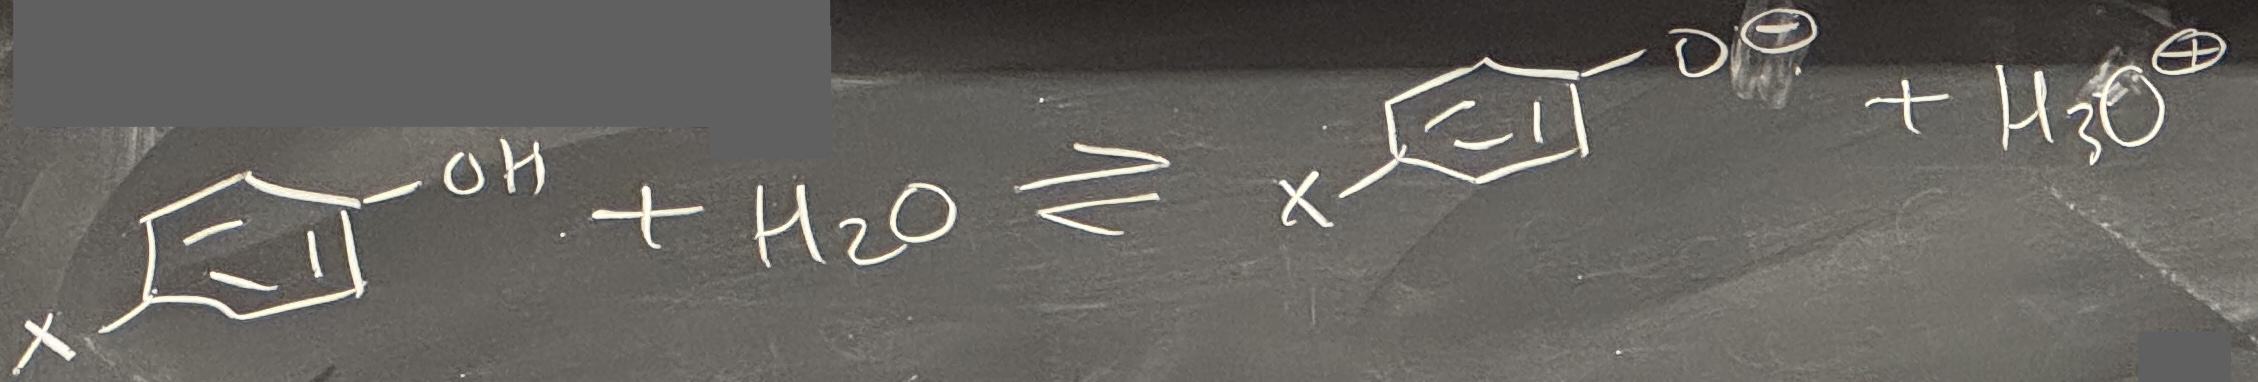
\includegraphics[width=0.9\linewidth]{rhoExa.JPG}
            \caption{Phenol deprotonation ($\rho=2.26$).}
            \label{fig:rhoExa}
        \end{subfigure}
        \begin{subfigure}[b]{0.49\linewidth}
            \centering
            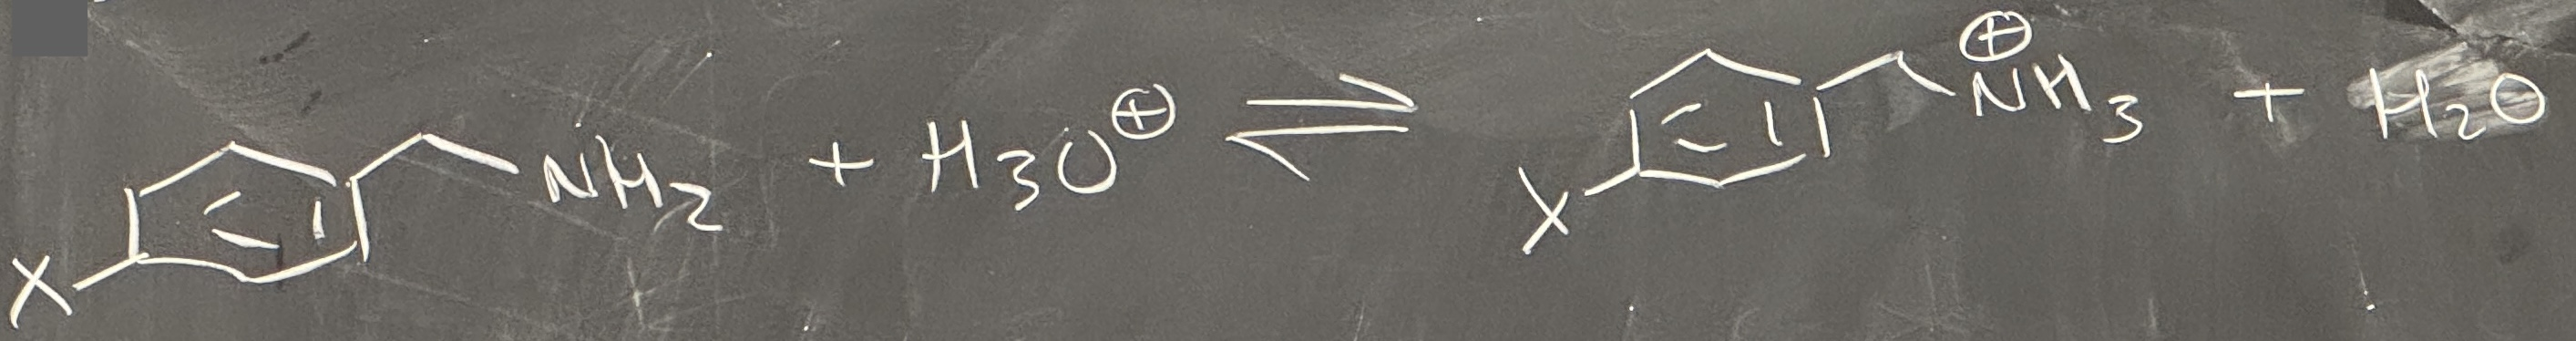
\includegraphics[width=0.95\linewidth]{rhoExb.JPG}
            \caption{Benzylamine protonation ($\rho=-1.05$).}
            \label{fig:rhoExb}
        \end{subfigure}\\[2em]
        \begin{subfigure}[b]{0.49\linewidth}
            \centering
            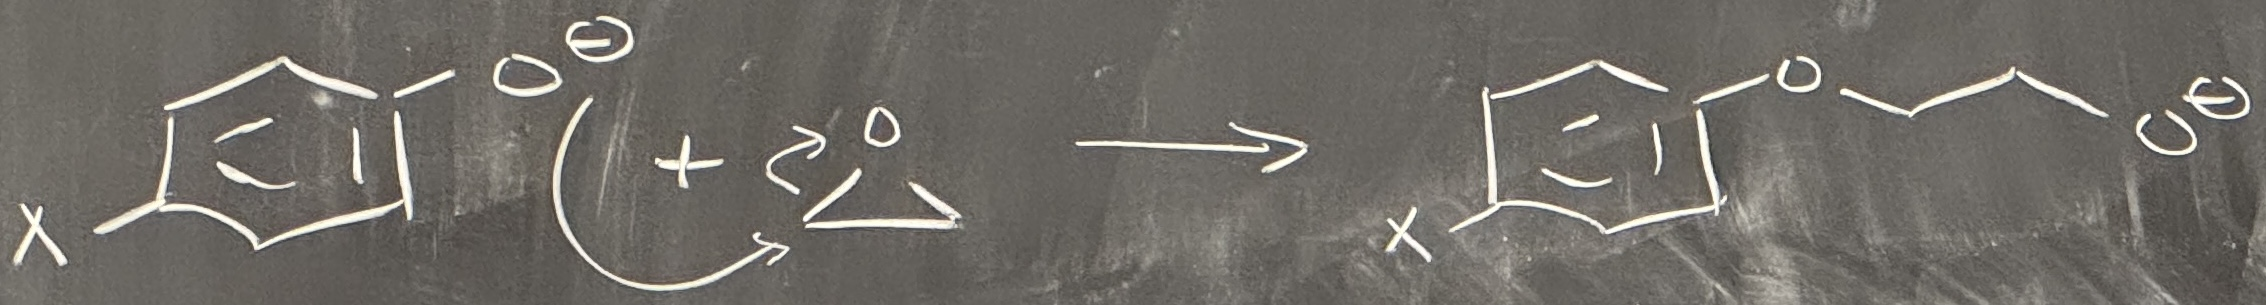
\includegraphics[width=0.95\linewidth]{rhoExc.JPG}
            \caption{Phenolate attack ($\rho=-0.95$).}
            \label{fig:rhoExc}
        \end{subfigure}
        \begin{subfigure}[b]{0.49\linewidth}
            \centering
            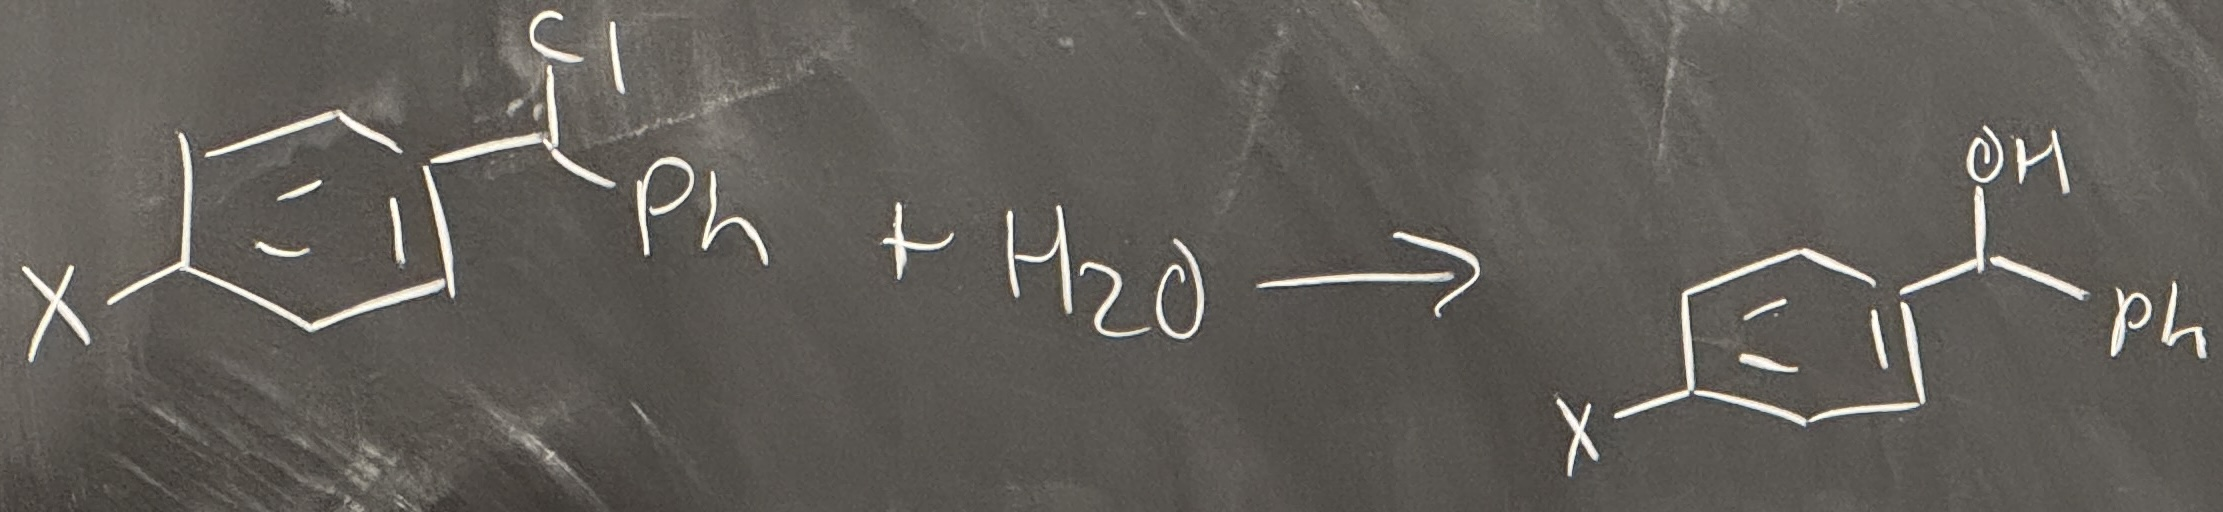
\includegraphics[width=0.8\linewidth]{rhoExd.JPG}
            \caption{Nucleophilic substitution ($\rho=-5.09$).}
            \label{fig:rhoExd}
        \end{subfigure}
        \caption{Sensitivity factors for simple reactions.}
        \label{fig:rhoEx}
    \end{figure}
    \begin{itemize}
        \item The deprotonation of \emph{para}-substituted phenols (Figure \ref{fig:rhoExa}).
        \begin{itemize}
            \item $\rho=2.26$.
            \item This means that we're building up negative charge in the transition state, and the reaction is more sensitive to \ce{X} than the reference reaction.
        \end{itemize}
        \item The protonation of \emph{para}-substituted benzylamines (Figure \ref{fig:rhoExb}).
        \begin{itemize}
            \item $\rho=-1.05$.
            \item This means that we're building up positive charge in the transition state.
        \end{itemize}
        \item The ring-opening backside attack of \emph{para}-substituted phenolates on epoxides (Figure \ref{fig:rhoExc}).
        \begin{itemize}
            \item $\rho=-0.95$.
            \item There's no discrete build up of positive charge in this reaction, but this value indicates that we have a loss of negative charge in the transition state.
        \end{itemize}
        \item A nucleophilic substitution (Figure \ref{fig:rhoExd}).
        \begin{itemize}
            \item $\rho=-5.09$.
            \item Since $\rho=-$, we're building up positive charge in the transition state.
            \item Since $|\rho|>1$, we're (significantly) more sensitive to substituents than the reference.
            \item These two facts can actually help us determine the mechanism of this reaction!
            \begin{itemize}
                \item There are two possible mechanisms by which this reaction can proceed: S\textsubscript{N}1 and S\textsubscript{N}2.
                \item The RDS of S\textsubscript{N}1 is the departure of the leaving group, and S\textsubscript{N}2 is concerted. Importantly, this means that S\textsubscript{N}1 mechanisms have a significantly greater buildup of positive charge in the "transition state" since they form a true carbocation.
                \item So since substituents have a \emph{significant} effect here, the mechanism of this particular nucleophilic substitution must be S\textsubscript{N}1!
                \item If it were S\textsubscript{N}2, we'd expect a small negative $\rho$.
            \end{itemize}
        \end{itemize}
        \item Takeaway: Sometimes Hammett plots give us simple insights, and sometimes they are powerful tools to help us probe reaction mechanisms.
        \begin{itemize}
            \item Usually, we measure $\rho$ and try to propose mechanisms that would be consistent with that $\rho$ value; we do not usually draw the mechanism and guess the $\rho$.
        \end{itemize}
    \end{itemize}
    \item While linear Hammett plots can evidently be very helpful, sometimes we get nonlinear relationships. These can also give us important information.
    \item Example: Consider the following two-step reaction.
    \begin{figure}[h!]
        \centering
        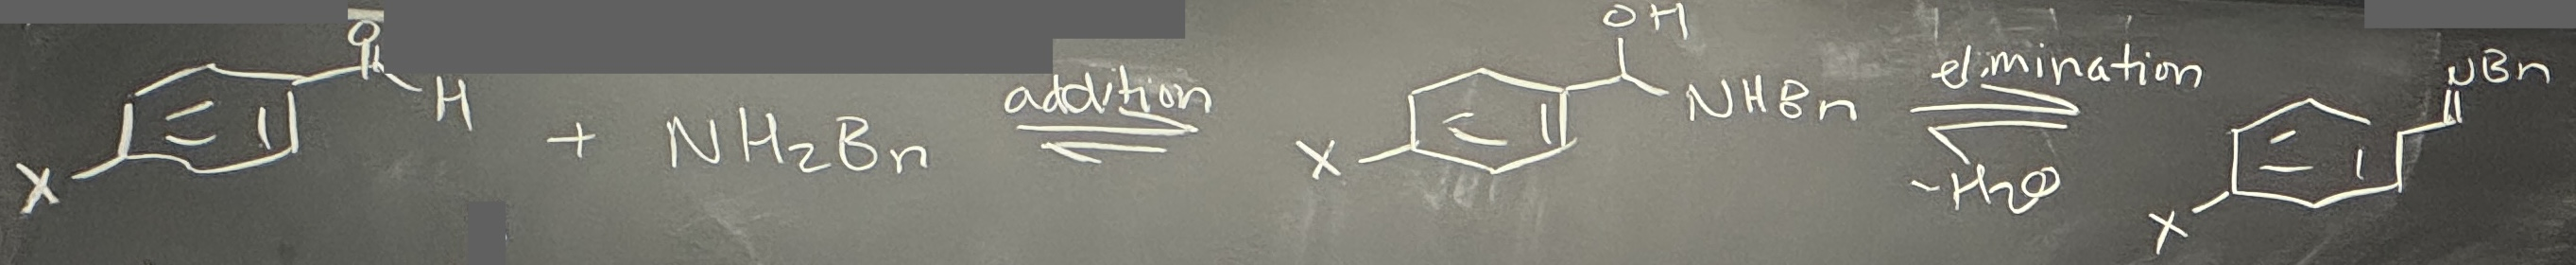
\includegraphics[width=0.8\linewidth]{imineSub.JPG}
        \caption{Imine formation from a substituted aldehyde.}
        \label{fig:imineSub}
    \end{figure}
    \begin{itemize}
        \item This is nucleophilic addition to an aldehyde, forming a hemiaminal, followed by elimination to the imine.
    \end{itemize}
    \item The Hammett plot for Figure \ref{fig:imineSub} is \textbf{concave down}.
    \begin{figure}[h!]
        \centering
        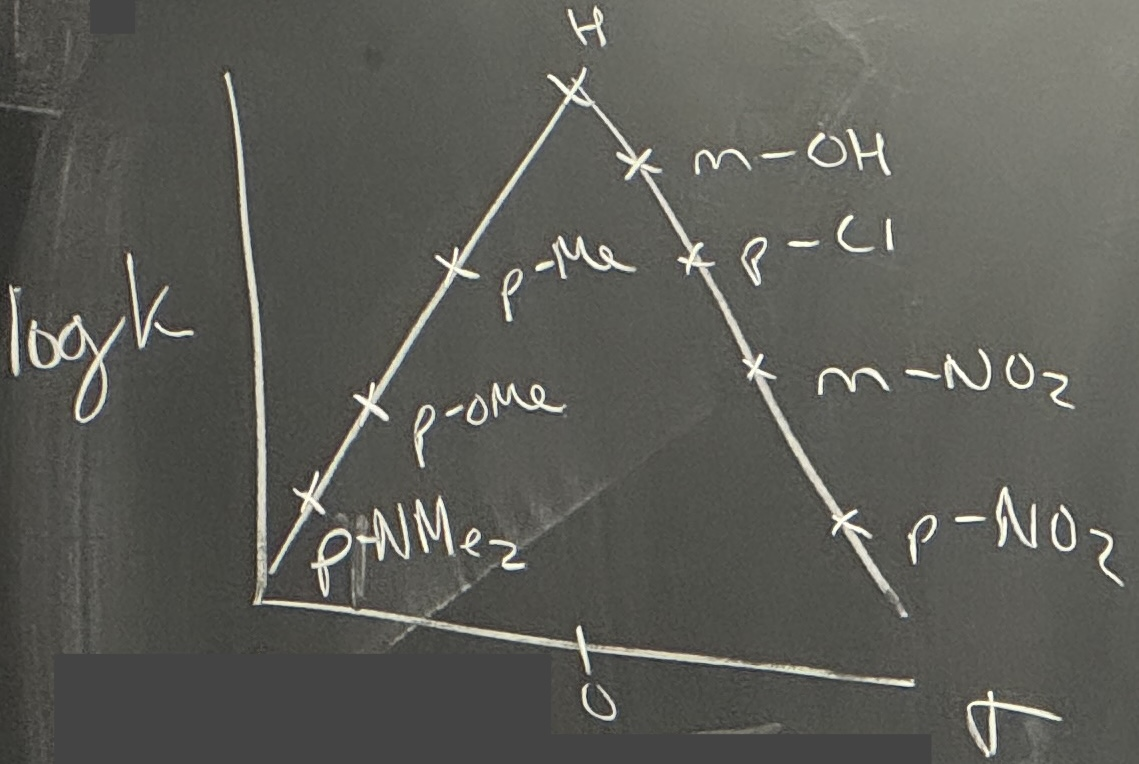
\includegraphics[width=0.35\linewidth]{HammettImine.JPG}
        \caption{Hammett plot for imine formation.}
        \label{fig:HammettImine}
    \end{figure}
    \begin{itemize}
        \item Notice that this Hammett plot deals with rate ($\Delta G^\ddagger$) because the $y$-axis is in $\log(k)$, not $\log(K)$.
        \item Hence, this Hammett plot is under the control of two \emph{kinetic} regimes.
        \item In the left regime, stronger EDGs decrease the rate of reaction.
        \begin{itemize}
            \item Stronger EDGs will make the initial carbonyl less electrophilic.
            \item Thus, with stronger EDGs, addition becomes the rate-limiting step.
        \end{itemize}
        \item In the right regime, stronger EWGs decrease the rate of reaction.
        \begin{itemize}
            \item Stronger EWGs will make the initial carbonyl more electrophilic (speeding up addition), and they will destabilize the positive charge that builds up when the hydroxyl group is protonated before elimination.
            \item Thus, with stronger EWGs, elimination becomes the rate-limiting step.
        \end{itemize}
    \end{itemize}
    \item \textbf{Concave down} (Hammett plot): A Hammett plot that indicates a change in rate-determining step as \ce{X} is varied, but the same overall mechanism.
    \begin{itemize}
        \item It should also make intuitive sense that a concave down plot changes the RDS: We have something of an equilibrium at \ce{H} and all we need is one step slowed down to be the RDS, so pushing one way slows down one step, and pushing the other way slows down the other step!
        \item Essentially, regardless of which step is accelerated or slowed down by EWGs/EDGs, what matters is that \emph{one} of the steps will be being slowed down, and \emph{that} step will become rate-limiting.
    \end{itemize}
    \item Further examples of concave down Hammett plots.
    \begin{figure}[h!]
        \centering
        \begin{subfigure}[b]{0.2\linewidth}
            \centering
            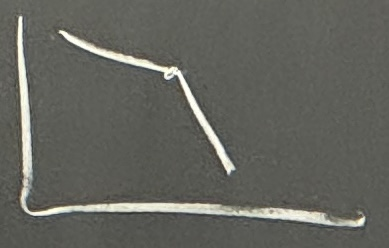
\includegraphics[width=0.7\linewidth]{HammettConcaveDa.JPG}
            \caption{Down-down.}
            \label{fig:HammettConcaveDa}
        \end{subfigure}
        \begin{subfigure}[b]{0.2\linewidth}
            \centering
            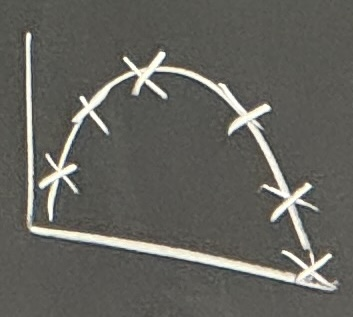
\includegraphics[width=0.5\linewidth]{HammettConcaveDb.JPG}
            \caption{Curved.}
            \label{fig:HammettConcaveDb}
        \end{subfigure}
        \caption{More concave down Hammett plots.}
        \label{fig:HammettConcaveD}
    \end{figure}
    \begin{itemize}
        \item Some can have two conjoined downward-sloped lines (Figure \ref{fig:HammettConcaveDa}).
        \begin{itemize}
            \item This also corresponds to a change in the RDS, but in this case, \emph{both} steps build up positive charge and hence are decelerated by EWGs.
        \end{itemize}
        \item Some can be curved down (Figure \ref{fig:HammettConcaveDb}).
        \begin{itemize}
            \item This corresponds to a more gradual change in RDS.
            \item We see this when the transition state "moves" with the substituent changes.
        \end{itemize}
    \end{itemize}
    \item This concludes our discussion of concave down Hammett plots.
    \item We now look at another example reaction and its Hammett plot.
    \begin{figure}[H]
        \centering
        \footnotesize
        \begin{subfigure}[b]{\linewidth}
            \centering
            \schemestart
                \chemfig{*6((-X)=-=(-(=[2]O)-[:-30]OMe)-=-)}
                \arrow{<=>[\ce{H+}][\ce{MeOH}]}[,1.2]
                \chemfig{*6((-X)=-=(-~\charge{[extra sep=4pt]0=$\oplus$}{O})-=-)}
                \arrow{<=>[\ce{H2O}][\ce{H+}]}[,1.2]
                \chemfig{*6((-X)=-=(-(=[2]O)-[:-30]OH)-=-)}
            \schemestop
            \caption{Methyl ester.}
            \label{fig:EsterHyda}
        \end{subfigure}\\[2em]
        \begin{subfigure}[b]{\linewidth}
            \centering
            \schemestart
                \chemfig{*6((-X)=-=(-(=[2]O)-[:-30]OEt)-=-)}
                \arrow{<=>[\ce{H+}][\ce{EtOH}]}[,1.2]
                \chemfig{*6((-X)=-=(-~\charge{[extra sep=4pt]0=$\oplus$}{O})-=-)}
                \arrow{<=>[\ce{H2O}][\ce{H+}]}[,1.2]
                \chemfig{*6((-X)=-=(-(=[2]O)-[:-30]OH)-=-)}
            \schemestop
            \caption{Ethyl ester (elimination-addition).}
            \label{fig:EsterHydb}
        \end{subfigure}\\[2em]
        \begin{subfigure}[b]{\linewidth}
            \centering
            \schemestart
                \chemfig{*6((-X)=-=(-(=[2]O)-[:-30]OEt)-=-)}
                \arrow{<=>[\ce{H+}]}[,1.4]
                \chemfig{*6((-X)=-=(-(=[2]O)-[:-30]@{2O}\chembelow{\charge{[extra sep=5pt]90=$\oplus$}{O}}{H}-[@{21}]@{2C}-[:-30])-=-)}
                \arrow{<=>[\chemfig{H_2@{3O}\charge{90=\:}{O}}][\ce{EtOH2+}]}[,1.4]
                \chemfig{*6((-X)=-=(-(=[2]O)-[:-30]OH)-=-)}
            \schemestop
            \chemmove{
                \draw [curved arrow={5pt}{2pt}] (3O) to[out=90,in=30] (2C);
                \draw [curved arrow={2pt}{2pt}] (21) to[out=120,in=53,looseness=1.8] (2O);
            }
            \caption{Ethyl ester (S\textsubscript{N}2).}
            \label{fig:EsterHydc}
        \end{subfigure}
        \caption{Acid-catalyzed ester hydrolysis.}
        \label{fig:EsterHyd}
    \end{figure}
    \begin{itemize}
        \item When a methyl ester hydrolyzes under acidic conditions, there is only one possible mechanism: Protonation of \ce{OMe} followed elimination of methanol, forming an acylium ion, then addition of water followed by deprotonation to the acid (Figure \ref{fig:EsterHyda}).
        \begin{itemize}
            \item We call this an "elimination-addition mechanism."
        \end{itemize}
        \item However, when an \emph{ethyl} ester hydrolyzes under acidic conditions, it can follow one of two mechanisms.
        \begin{enumerate}
            \item An analogous elimination-addition mechanism (Figure \ref{fig:EsterHydb}).
            \item Protonation of the ester oxygen followed by an S\textsubscript{N}2-type mechanism (Figure \ref{fig:EsterHydc}).
        \end{enumerate}
    \end{itemize}
    \item The Hammett plot for the hydrolysis of a methyl ester is linear - down (Figure \ref{fig:HammettEstera}), but the Hammett plot for the hydrolysis of an ethyl ester is \textbf{concave up} (Figure \ref{fig:HammettEsterb}).
    \begin{figure}[h!]
        \centering
        \begin{subfigure}[b]{0.36\linewidth}
            \centering
            \begin{tikzpicture}[scale=2]
                \path ([xshift=-1.5cm]0.35,0) -- ([xshift=1.5cm]0.35,0);
                \small
                \draw (-0.5,1.2) -- node[left]{$\log(\tfrac{k_{\ce{X}}}{k_{\ce{H}}})$} (-0.5,-0.5) -- node[below]{$\sigma_{\ce{X}}$} (1.2,-0.5);
                
                \draw [rex,thick] (-0.4,0.4) -- (0.4,-0.4);
            \end{tikzpicture}
            \caption{Methyl ester.}
            \label{fig:HammettEstera}
        \end{subfigure}
        \begin{subfigure}[b]{0.36\linewidth}
            \centering
            \begin{tikzpicture}[scale=2]
                \path ([xshift=-1.5cm]0.35,0) -- ([xshift=1.5cm]0.35,0);
                \small
                \draw (-0.5,1.2) -- node[left]{$\log(\tfrac{k_{\ce{X}}}{k_{\ce{H}}})$} (-0.5,-0.5) -- node[below]{$\sigma_{\ce{X}}$} (1.2,-0.5);
                
                \draw [rex,thick] (-0.4,0.8) -- (0,0) -- (0.55,1.1);
            \end{tikzpicture}
            \caption{Ethyl ester.}
            \label{fig:HammettEsterb}
        \end{subfigure}
        \caption{Hammett plots for ester hydrolysis.}
        \label{fig:HammettEster}
    \end{figure}
    \begin{itemize}
        \item The hydrolysis of a methyl ester displays a constant, negative sensitivity factor (Figure \ref{fig:HammettEstera}).
        \begin{itemize}
            \item This is because the positively charged acylium ion intermediate gets destabilized by stronger EWGs.
        \end{itemize}
        \item The hydrolysis of an ethyl ester displays a negative sensitivity factor for EDGs, and a positive sensitivity factor for EWGs (Figure \ref{fig:HammettEsterb}).
        \begin{itemize}
            \item When \ce{X} is an EDG, the acylium ion get stabilized. Weaker EDGs stabilize it less ($\rho=-$), but we still favor the elimination-addition mechanism (Figure \ref{fig:EsterHydb}).
            \item When \ce{X} is an EWG, the carboxylic acid is a better leaving group (\ref{fig:EsterHydc}). This corresponds to a positive Hammett slope.
        \end{itemize}
    \end{itemize}
    \item \textbf{Concave up} (Hammett plot): A Hammett plot that indicates a change in mechanism.
    \begin{itemize}
        \item It should also make intuitive sense that a concave up plot changes the mechanism: Here, both EDGs and EWGs \emph{accelerate} a certain pathway. Thus, it doesn't matter if they're slowing the RDS of one mechanism; there's another that they accelerate!
        \item Essentially, regardless of which mechanism is accelerated or slowed down by EWGs/EDGs, what matters is that \emph{one} of the mechanisms is being accelerated, and \emph{that} mechanism becomes operative.
    \end{itemize}
    \item Why are neither of these mechanisms addition-elimination?
    \begin{itemize}
        \item That's better under basic conditions!
    \end{itemize}
    \item Take-home message: Any deviation from linearity in a Hammett plot indicates a change in the RDS or the mechanism.
    \item Hammett plots are a very powerful mechanistic tool; think about using them in your final mechanistic proposal!!
\end{itemize}




\end{document}